\normalsize
\section{Gravity Current Test}

The subject of gravity currents has examples of snow avalanches, pyroclastic flows, and transport phenomena in the atmosphere and the ocean as mentioned by Samothrakis \cite{Samothrakis2005}. Therefore, the gravity current simulation is chosen to test the receding boundary method. The setup is similar to the experiment conducted by Maxworthy et al. \cite{Maxworthy02}. At the left boundary of a tank, the fluid with higher salinity is released into the ambient fluid with linearly stratified salinity.



In the numerical model, the tank is $2.0 \ m$ long and $0.2 \ m$ wide. The bottom slope is zero. The water depth is $0.15 \ m$. A two-dimensional version is tested with the grid resolution set to be $NX \times NZ = 100 \times 40$ with $dx=0.02 (m)$ and $dz=0.005 (m)$.
The salinity in the fixed volume to be released is set to $112 (g/kg)$ and in the stratified fluid the salinity varies linearly from $39.5 (g/kg)$ at the bottom layer to zero at the surface layer.
The computational time step $dt$ is set to be $0.005 (sec)$. The viscosity is specified as $10^{-6} (m^2/s)$. The tolerance of the pressure-Poisson solver is set to satisfy the maximum divergence error of each computational step: $\di \+u < 10^{-5} (1/sec)$. The simulation result without the receding boundary method is plotted in Fig. \ref{fig:RBM-GC-1Domain}.

For the implementation of the receding boundary method, the whole domain ($NX \times NZ = 100 \times 40$) is decomposed into two subdomains with $X_{mid} = 50$ and $B=24$. In other words, the left-hand-side subdomain spans, in the $x$-axis direction, from the first grid to the 74th grid\footnote[1]{$X_{mid} + B = 74$}, and the right-hand-side subdomain spans from the 26th grid\footnote[2]{$X_{mid} - B = 26$} to the $100th$ grid.

The receding rate is tested from $G=1$ to $G=3$. With the receding rate $G=1$, the subiteration $S$ is tested from $S=2$ to $S=12$; with $G=2$, the subiteration $S$ is tested from $S=3$ to $S=12$; with $G=3$, the subiteration $S$ is tested from $S=3$ to $S=8$.
The simulation result of the case $G=2$ and $S=10$ is shown in Fig. \ref{fig:RBM-GC-2Domain-S10-B24-G2-660}. The receding boundary in action can be seen in Fig. \ref{fig:RBM-GC-2Domain-R-S10-B24-G2-660} for the right-hand-side subdomain and Fig. \ref{fig:RBM-GC-2Domain-L-S10-B24-G2-660} for the left-hand-side subdomain.

The difference between the simulations with and without RBM is quantified by the $L_1$ and $L_2$ norms,
\be
error_1=\sqrt{\f{\sum_{i=1}^{N} |x_i-y_i|}{N}}
\ee
\be
error_2=\sqrt{\f{\sum_{i=1}^{N} (x_i-y_i)^2}{N}}
\ee
Both are then normalized by the range between maximum and minimum value of the variables at that time step without RBM. The normalized average deviation is:
\be
error_1^*= error_1/(y_{max}-y_{min})
\ee
The normalized Root Mean Square is:
\be
error_2^*=error_2/(y_{max}-y_{min})
\ee

The simulation plots without RBM (Fig. \ref{fig:RBM-GC-1Domain}) and with RBM (Fig. \ref{fig:RBM-GC-2Domain-S10-B24-G2-660}) are very similar. This small difference is further confirmed in the analysis of the normalized deviation and root-mean-square. For the case of receding rate $G=2$ with different subiteration $S$, the normalized root-mean-square of the density difference ranges from 0.3\% of to 0.9\%, the pressure 0.2\% of to 1.1\%, the horizontal velocity 0.2\% to 1\%, and the vertical velocity 0.13\% to 0.4\%.

It's interesting that with the same buffer($B=24$), the higher subiteration $S$ does not necessarily result in greater discrepancy. As can be seen in Fig. \ref{fig:RBM-GC-den-error-G2-B24}, the density error 0.4\% of $S=10$ is smaller than 0.9\% of $S=6$ and 0.7\% of $S=5$.
To further investigate this behavior, the buffer is tested from $B=12$ to $B=24$. The time-averaged root-mean-square of the density error in Fig. \ref{fig:RBM-Den-Error-G2} shows the trend of increasing discrepancy with increasing buffer $B$. The fluctuation of the errors for different subiteration $S$ could be due to the linear smoothing (Section \ref{chapter:RBM-Smoothing}) of the essentially non-linear Navier-Stokes equation. The discussion of optimized smoother is beyond this work's scope but the development could possibly lower the errors and improve the consistency for different subiterations.

As shown in Table \ref{tab:RBM-computation-time} and Fig \ref{fig:RBM-Den-Error-G2}, the serial computation time of the gravity current simulations with RBM is around 25\% to 50\% more than that without RBM. These tests are performed on a 3.0GH Pentium IV PC with 2GB memory. The increased computation time is probably due to the increased total domain size resulted from the overlapping of subdomains. Since the RBM features the independent solution of each subdomain with information exchange only occurs at the subdomain boundary reset step, future research will include the implementation of the parallel version to take this advantage.

A three-dimensional version of the gravity simulation with RBM is still under development. One successful run with two subdomains is demonstrated in Fig. \ref{fig:RBM-3D-comparison} which shows the simulation results with and without the RBM, and in Fig \ref{fig:RBM-3D-action} which shows the boundary receding in action.



 \begin{figure}[htbp]
  \begin{center}
\includegraphics[scale=0.35]{../figures/Exp3-CASE1-dt0.005/OneDomain/01.pdf} 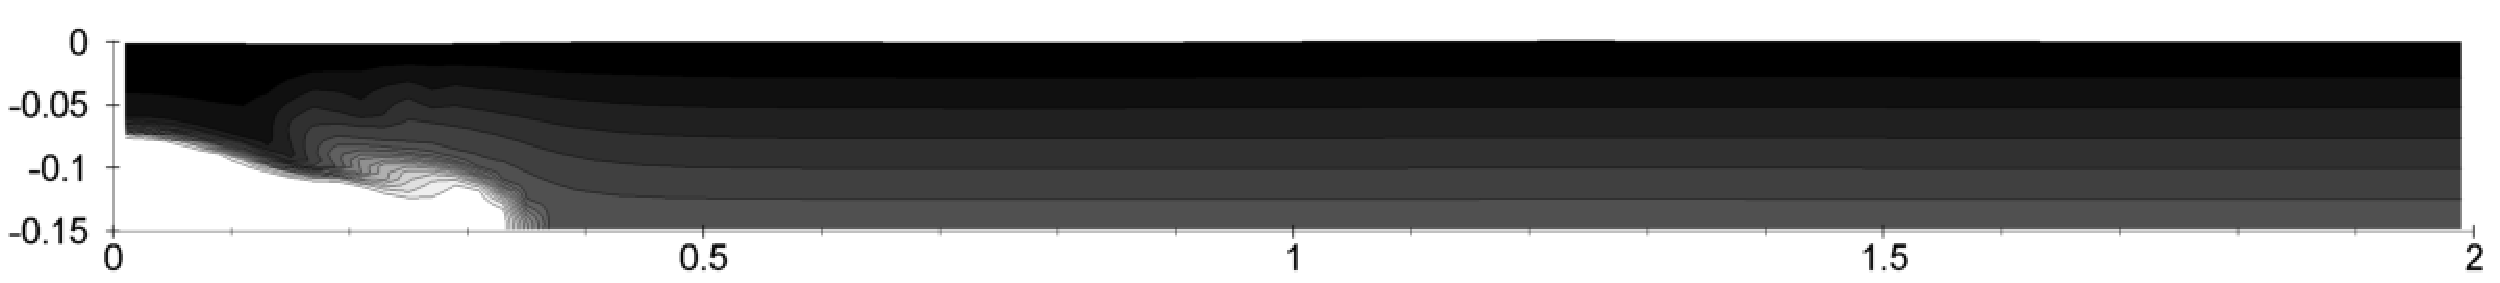
\includegraphics[scale=0.35]{../figures/Exp3-CASE1-dt0.005/OneDomain/03.pdf}
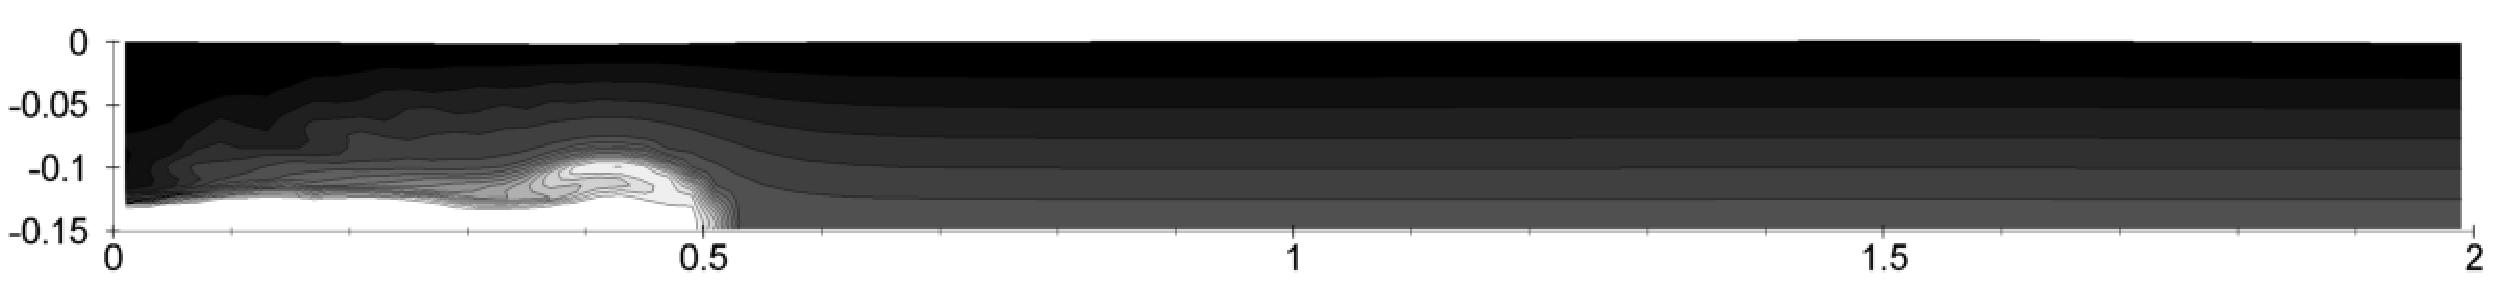
\includegraphics[scale=0.35]{../figures/Exp3-CASE1-dt0.005/OneDomain/05.pdf}
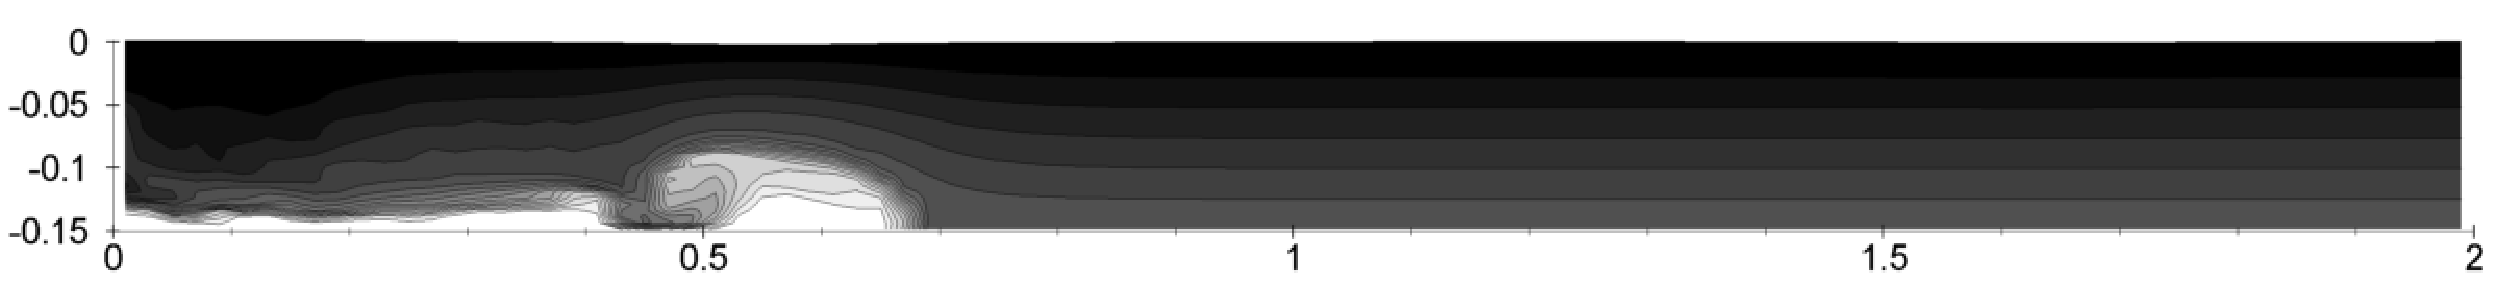
\includegraphics[scale=0.35]{../figures/Exp3-CASE1-dt0.005/OneDomain/07.pdf}
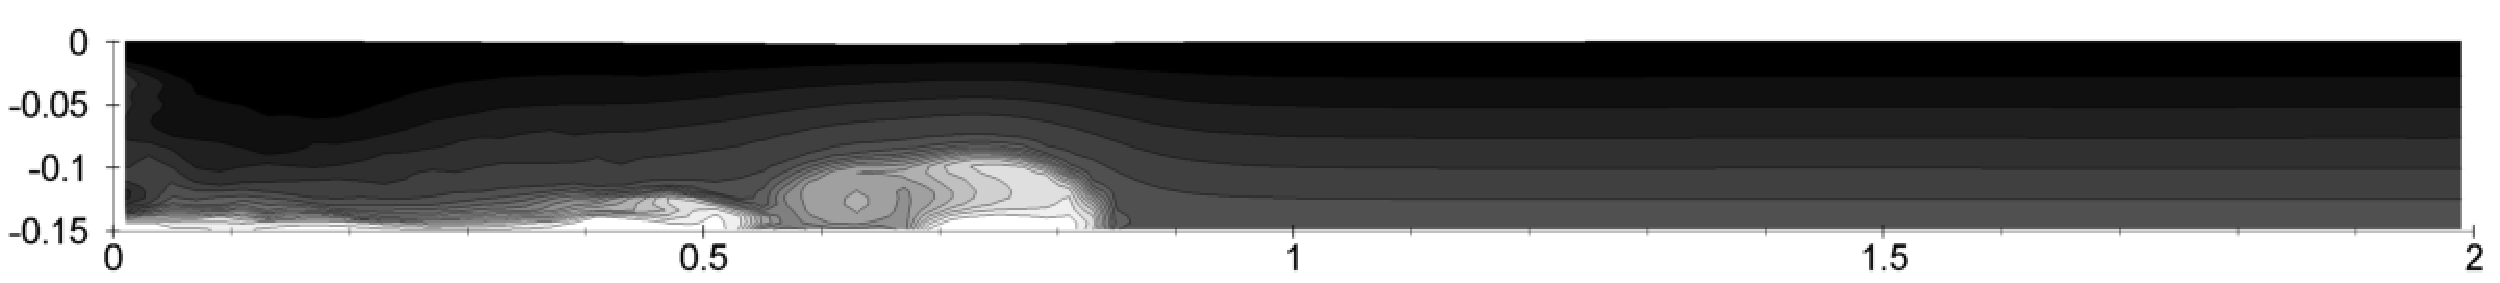
\includegraphics[scale=0.35]{../figures/Exp3-CASE1-dt0.005/OneDomain/09.pdf}
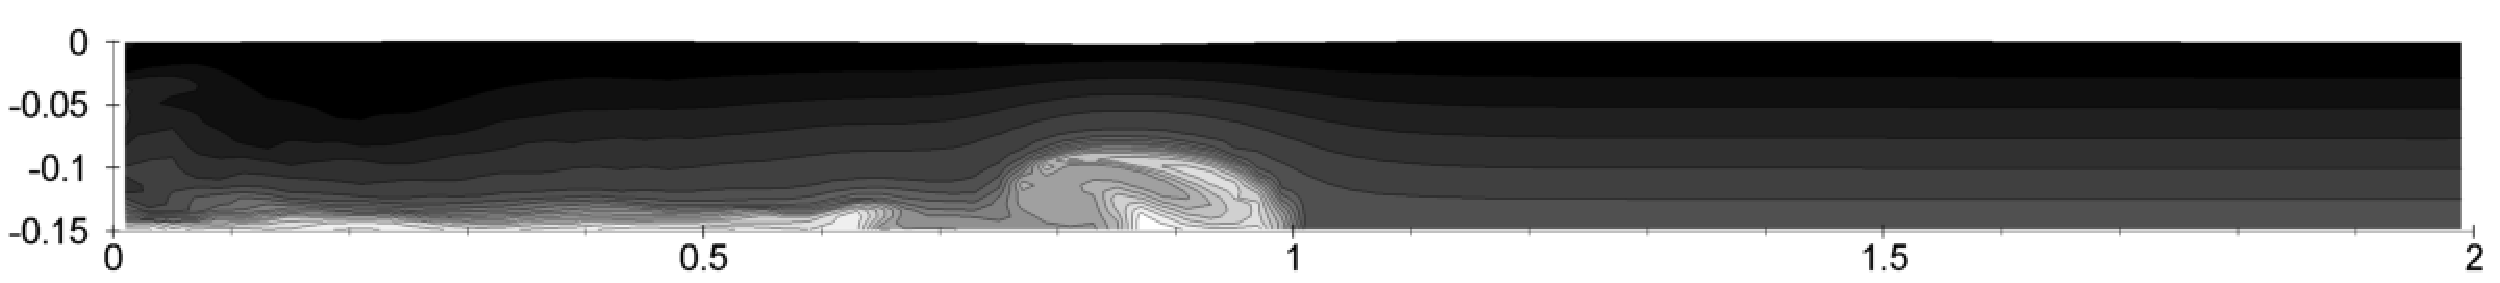
\includegraphics[scale=0.35]{../figures/Exp3-CASE1-dt0.005/OneDomain/11.pdf}
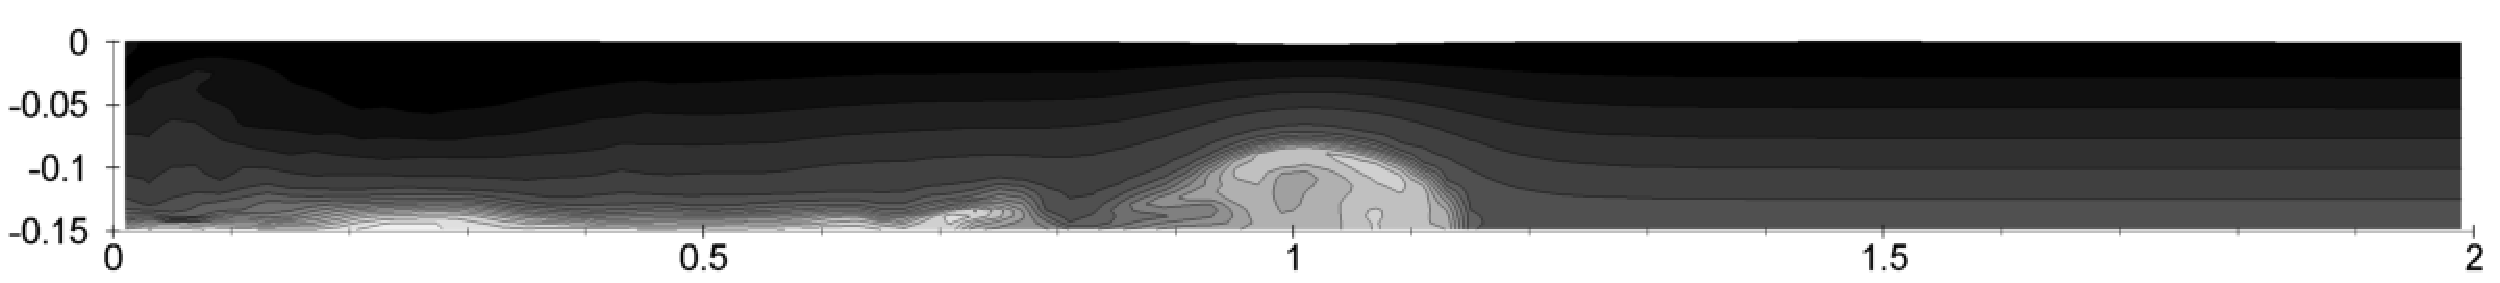
\includegraphics[scale=0.35]{../figures/Exp3-CASE1-dt0.005/OneDomain/13.pdf}
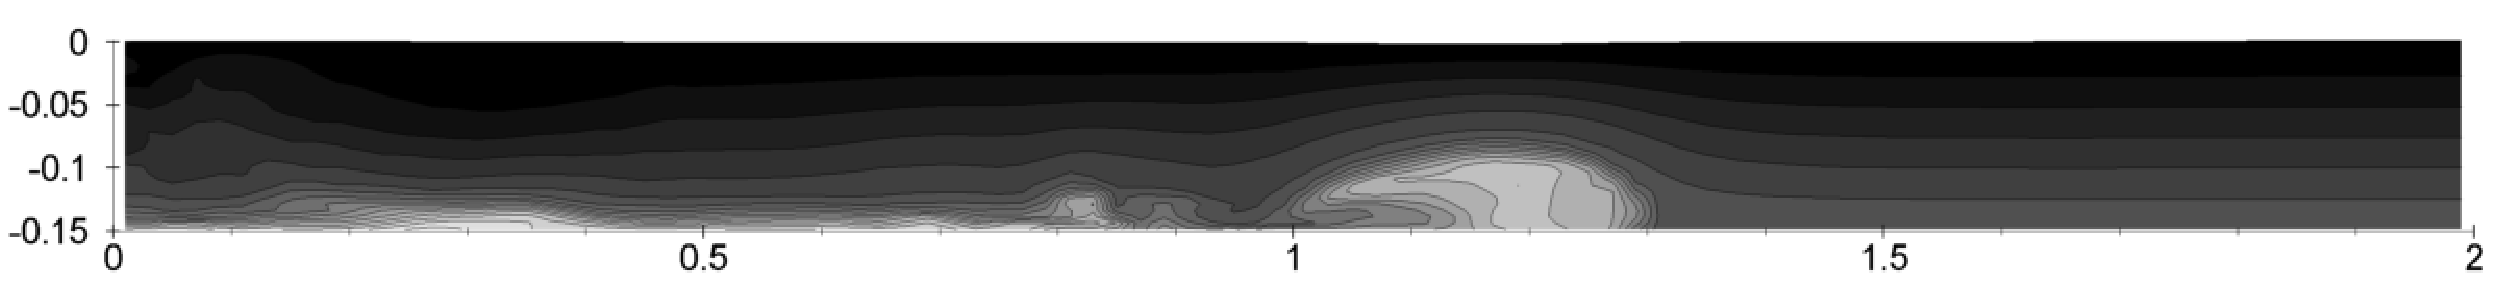
\includegraphics[scale=0.35]{../figures/Exp3-CASE1-dt0.005/OneDomain/15.pdf}
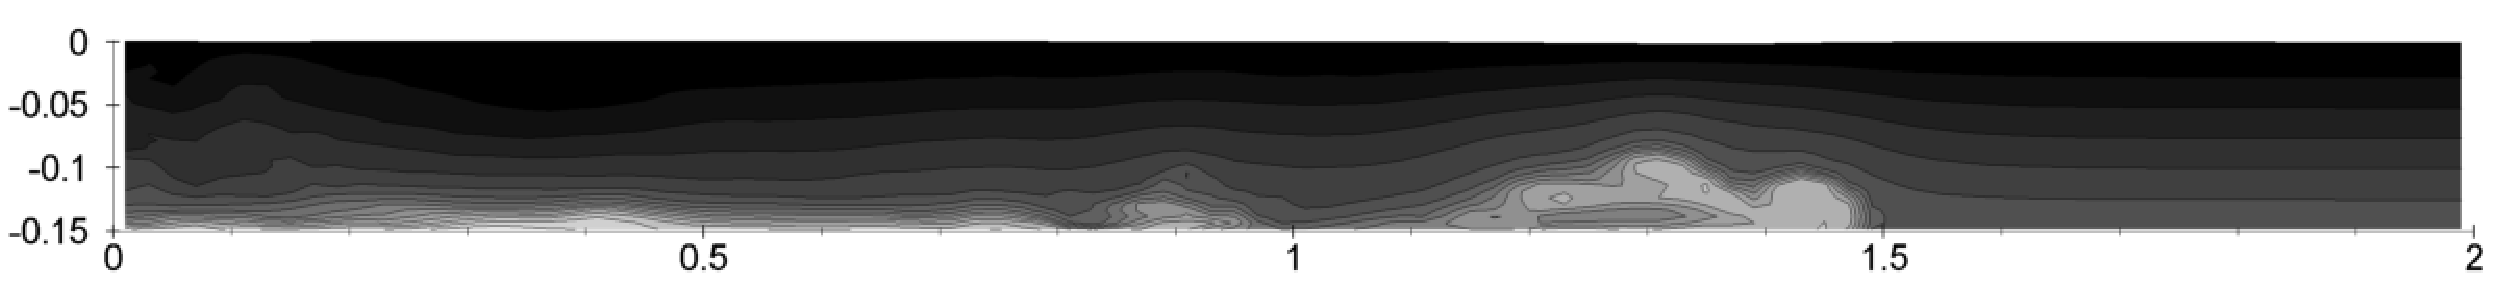
\includegraphics[scale=0.35]{../figures/Exp3-CASE1-dt0.005/OneDomain/17.pdf}
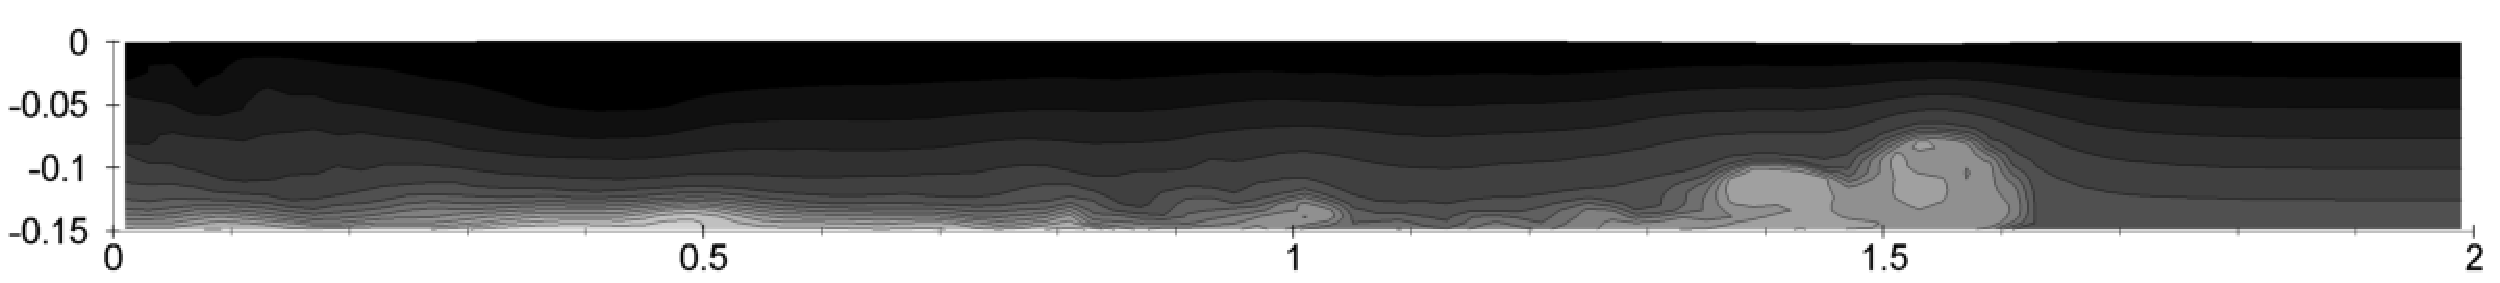
\includegraphics[scale=0.35]{../figures/Exp3-CASE1-dt0.005/OneDomain/19.pdf}
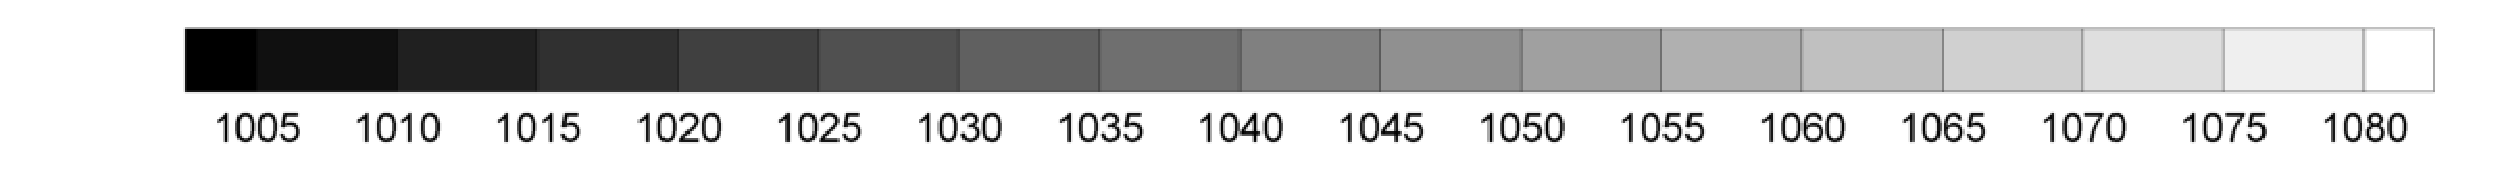
\includegraphics[scale=0.35]{../figures/Exp3-CASE1-dt0.005/legend.pdf}
    \caption{Gravity current simulation without RBM.}
    \label{fig:RBM-GC-1Domain}
  \end{center}
\end{figure}


\cp

\begin{figure}[htbp]
  \begin{center}    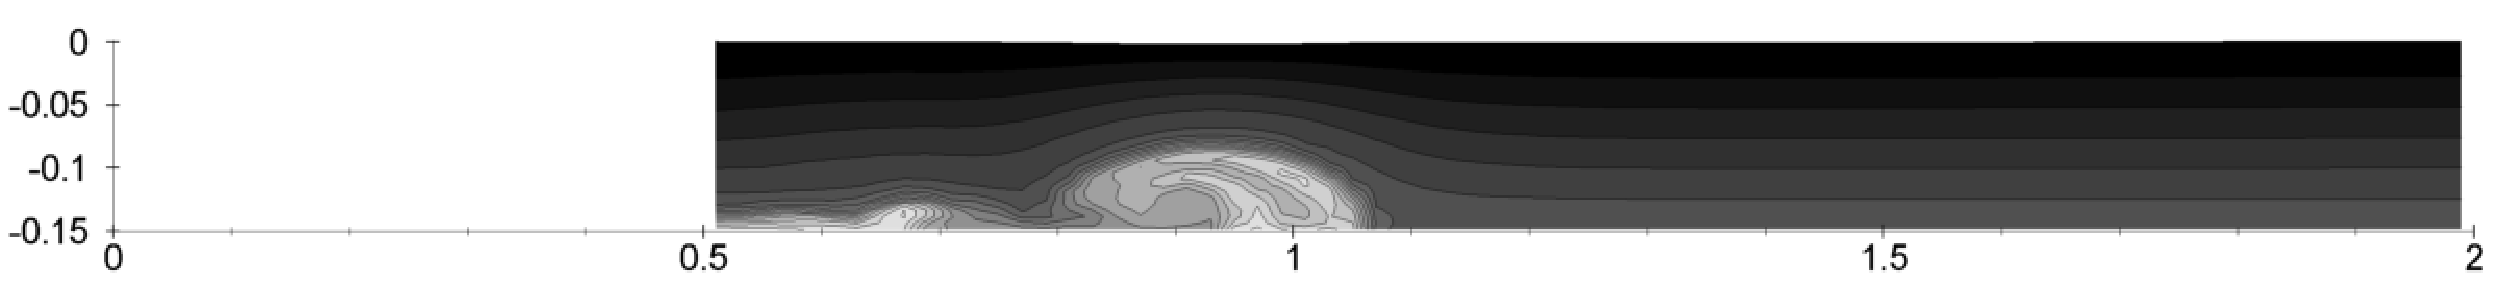
\includegraphics[scale=0.35]{../figures/Exp3-CASE1-dt0.005/rec_2_buf_24_sub_10/D1-101.pdf}
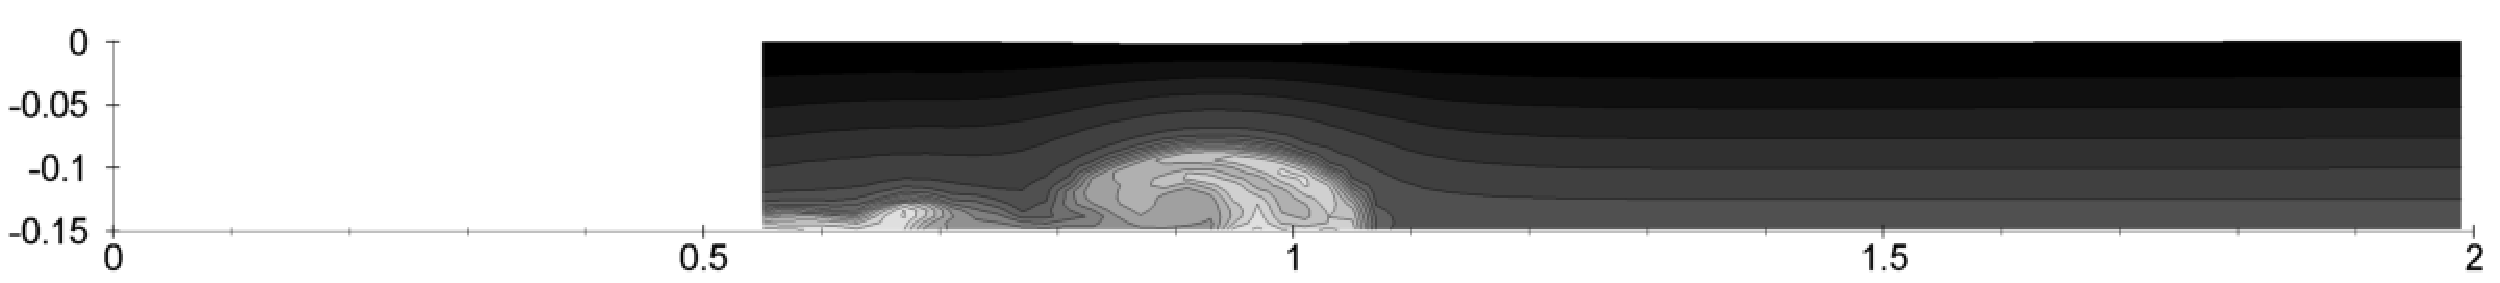
\includegraphics[scale=0.35]{../figures/Exp3-CASE1-dt0.005/rec_2_buf_24_sub_10/D1-102.pdf}
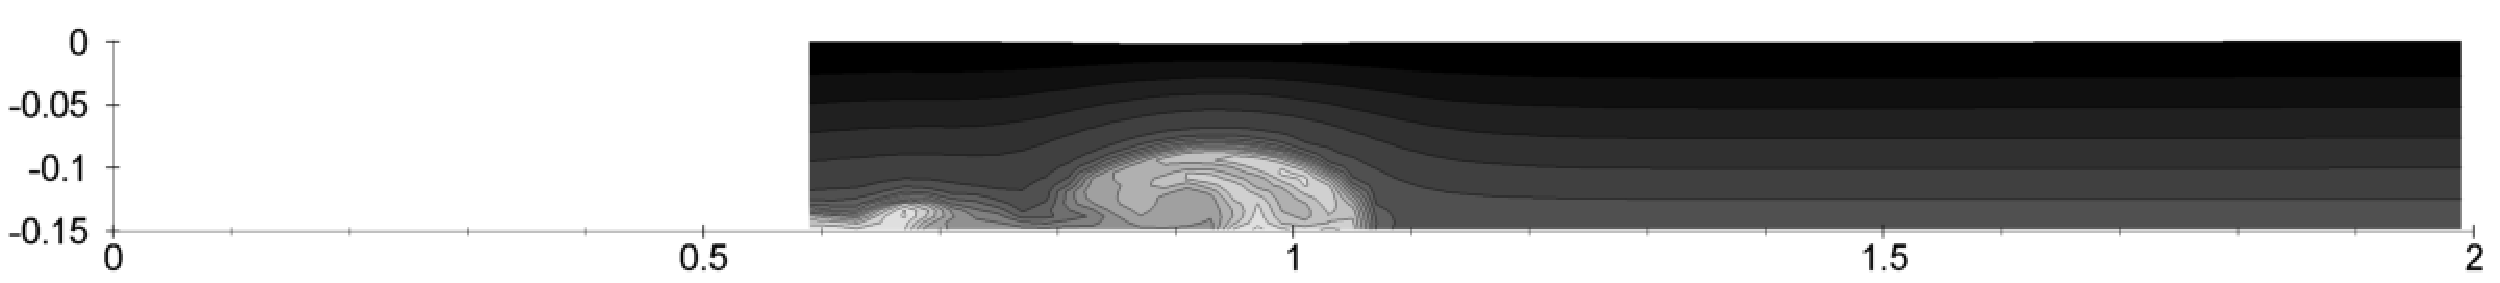
\includegraphics[scale=0.35]{../figures/Exp3-CASE1-dt0.005/rec_2_buf_24_sub_10/D1-103.pdf}
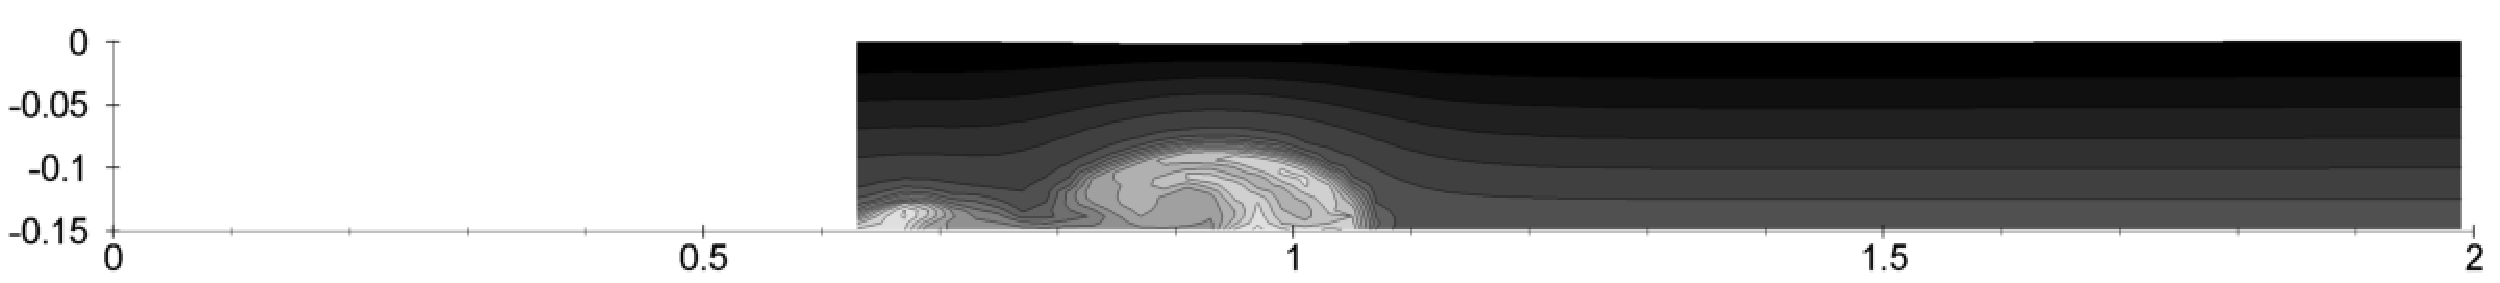
\includegraphics[scale=0.35]{../figures/Exp3-CASE1-dt0.005/rec_2_buf_24_sub_10/D1-104.pdf}
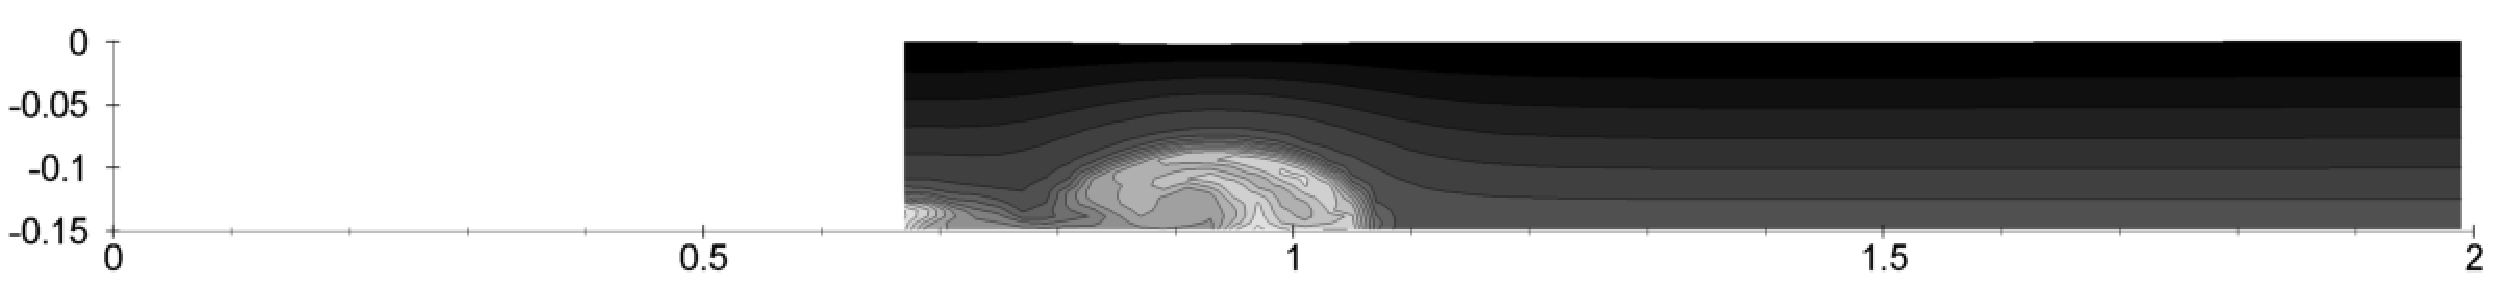
\includegraphics[scale=0.35]{../figures/Exp3-CASE1-dt0.005/rec_2_buf_24_sub_10/D1-105.pdf}
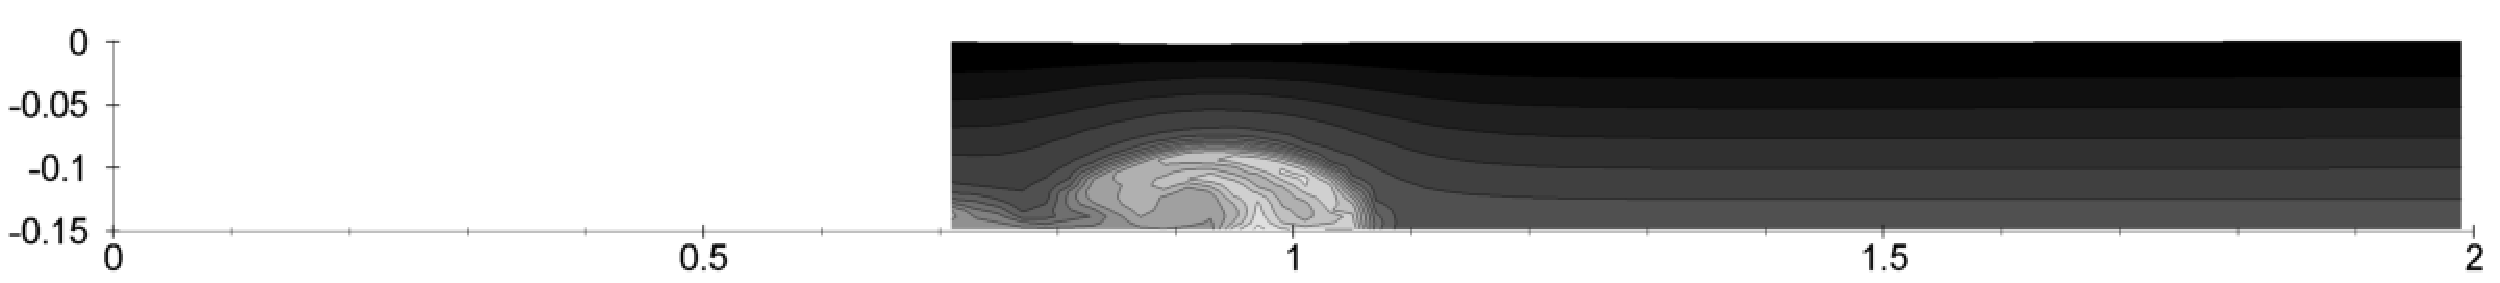
\includegraphics[scale=0.35]{../figures/Exp3-CASE1-dt0.005/rec_2_buf_24_sub_10/D1-106.pdf}
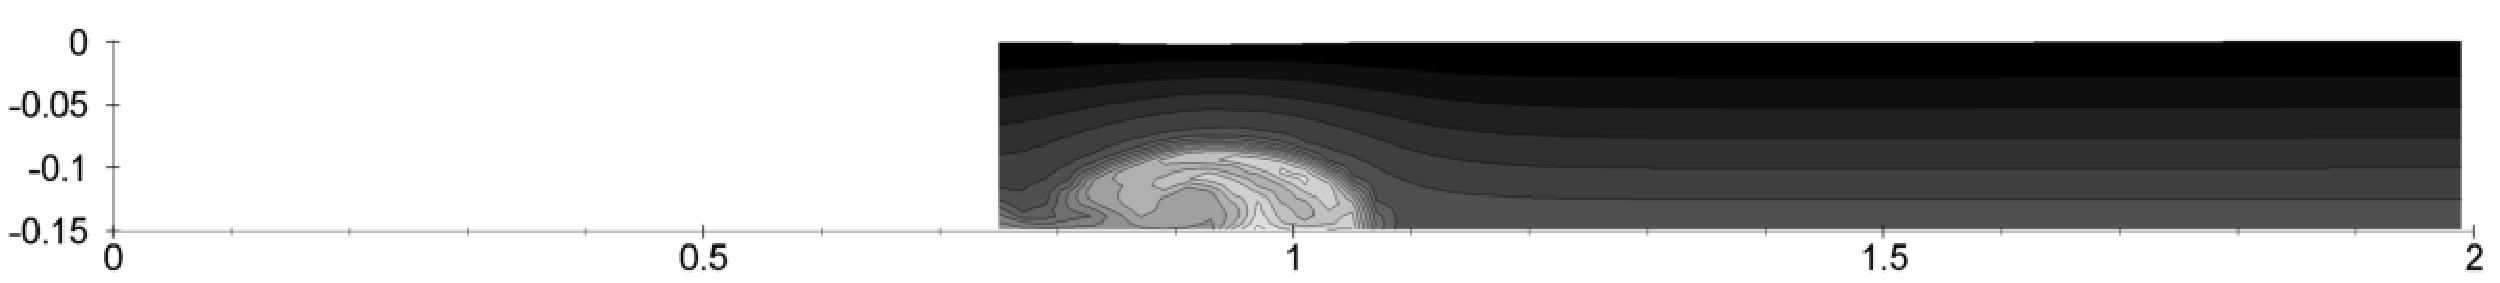
\includegraphics[scale=0.35]{../figures/Exp3-CASE1-dt0.005/rec_2_buf_24_sub_10/D1-107.pdf}
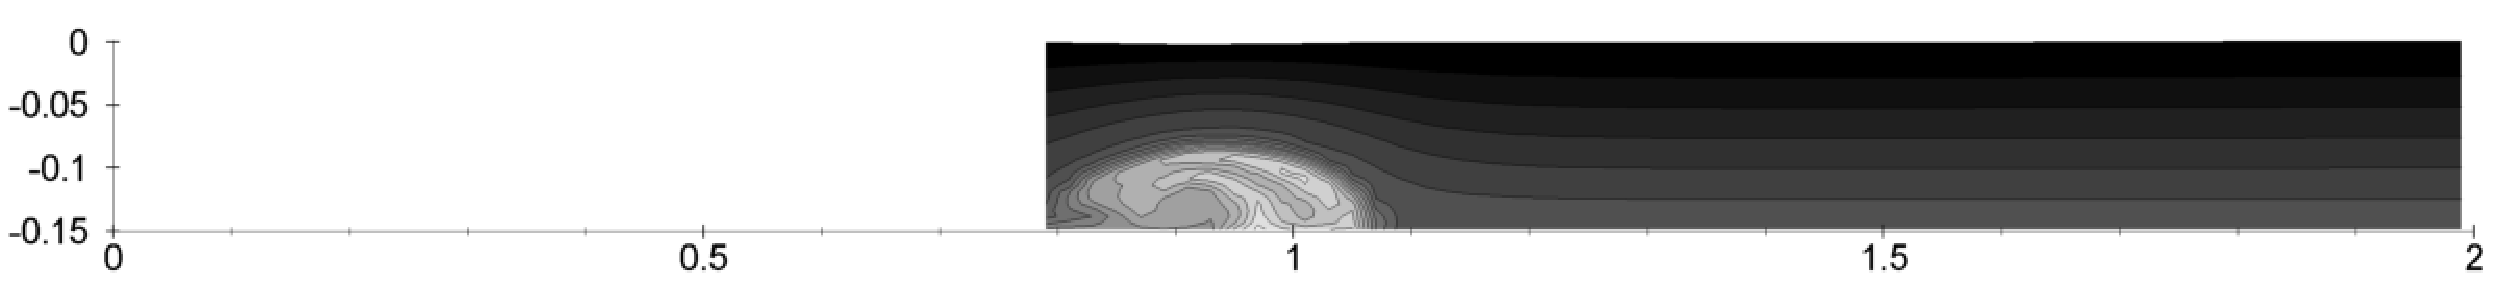
\includegraphics[scale=0.35]{../figures/Exp3-CASE1-dt0.005/rec_2_buf_24_sub_10/D1-108.pdf}
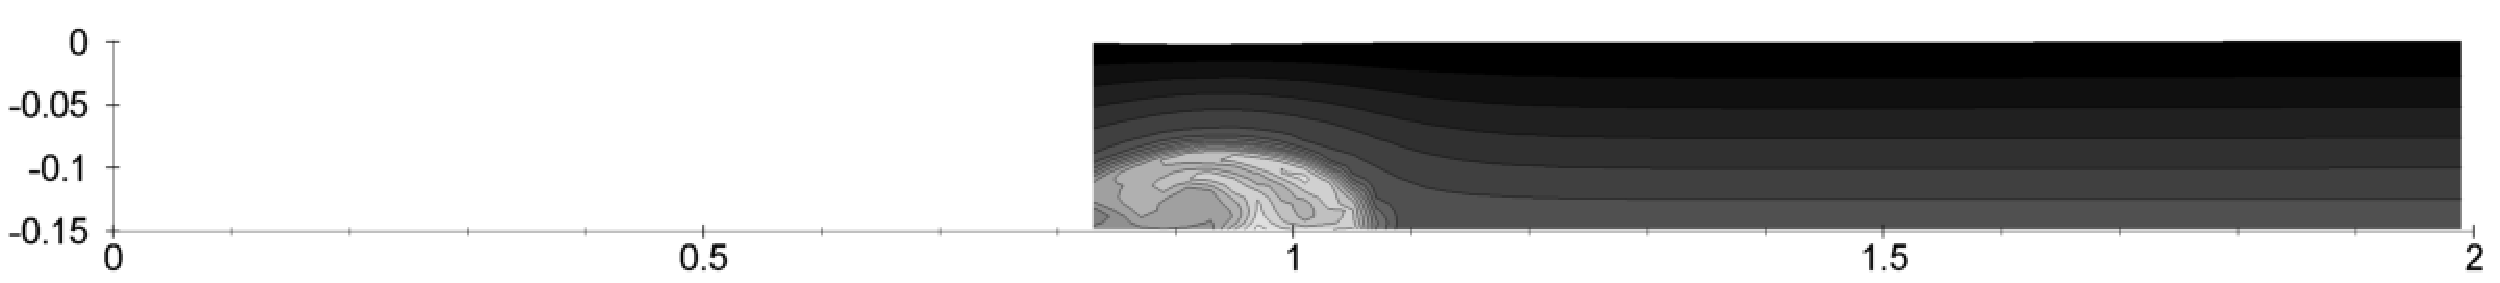
\includegraphics[scale=0.35]{../figures/Exp3-CASE1-dt0.005/rec_2_buf_24_sub_10/D1-109.pdf}
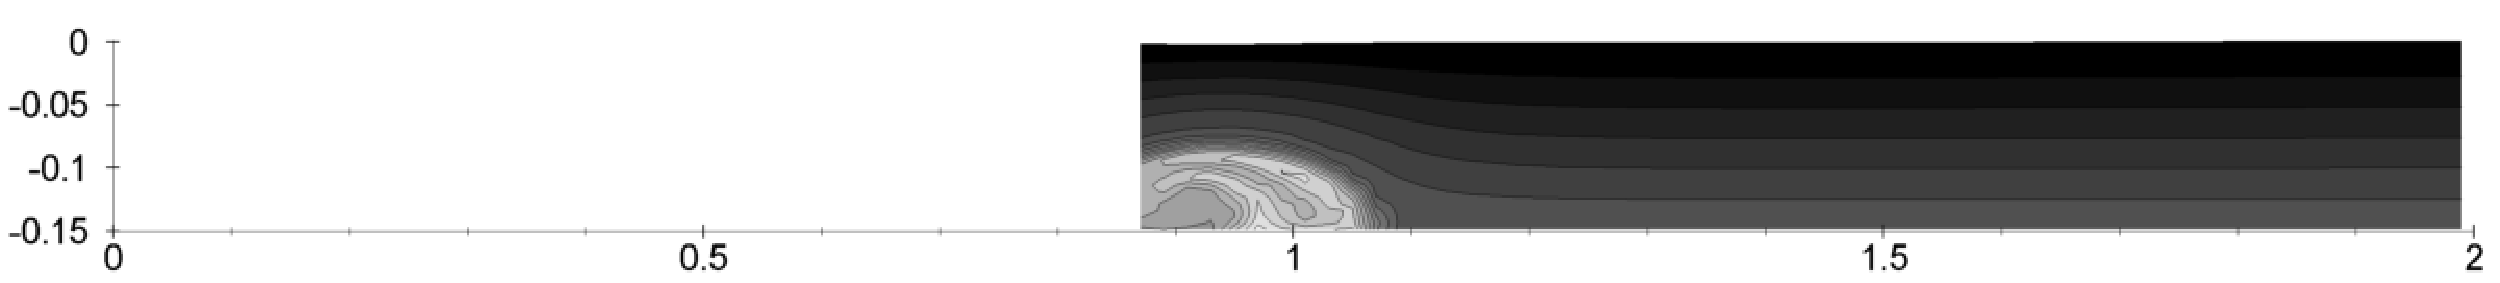
\includegraphics[scale=0.35]{../figures/Exp3-CASE1-dt0.005/rec_2_buf_24_sub_10/D1-110.pdf}
    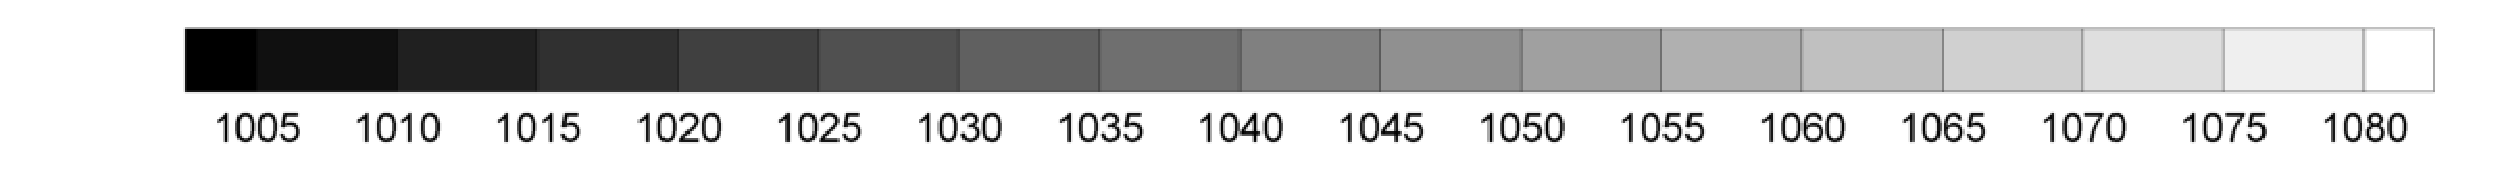
\includegraphics[scale=0.35]{../figures/Exp3-CASE1-dt0.005/legend.pdf}
    \caption{Gravity current simulation with RBM (S=10 B=24 G=2). The figures are the right-hand-side subdomain at $t=6.60-6.65(sec)$}
    \label{fig:RBM-GC-2Domain-R-S10-B24-G2-660}
  \end{center}
\end{figure}

\cp

\begin{figure}[htbp]
  \begin{center}    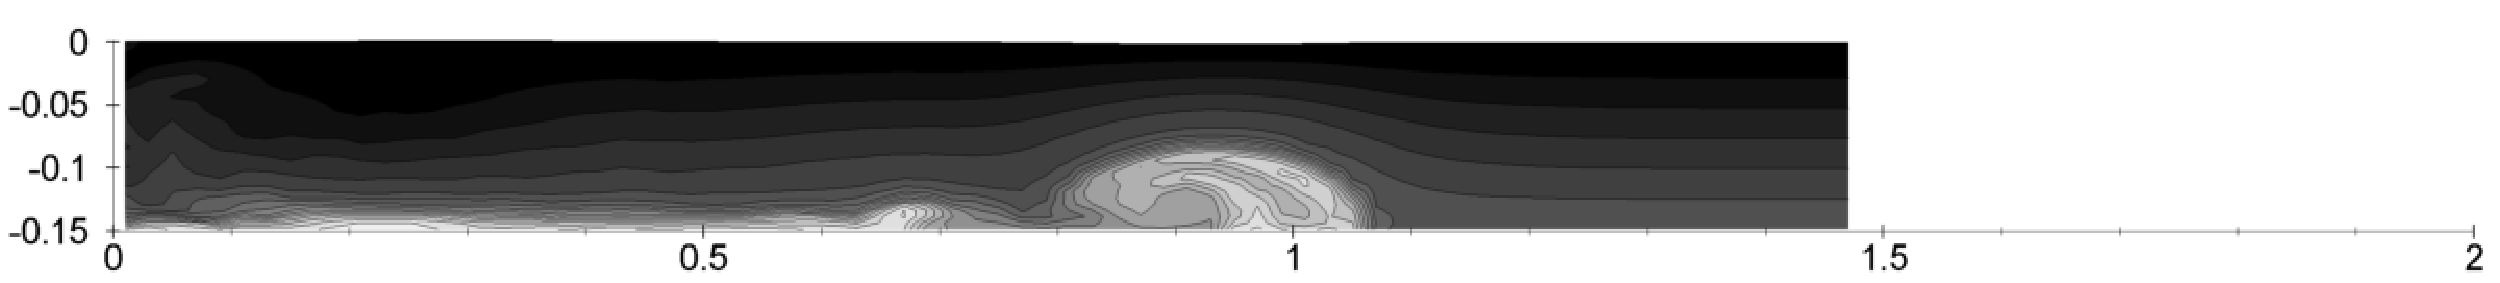
\includegraphics[scale=0.35]{../figures/Exp3-CASE1-dt0.005/rec_2_buf_24_sub_10/D2-101.pdf}
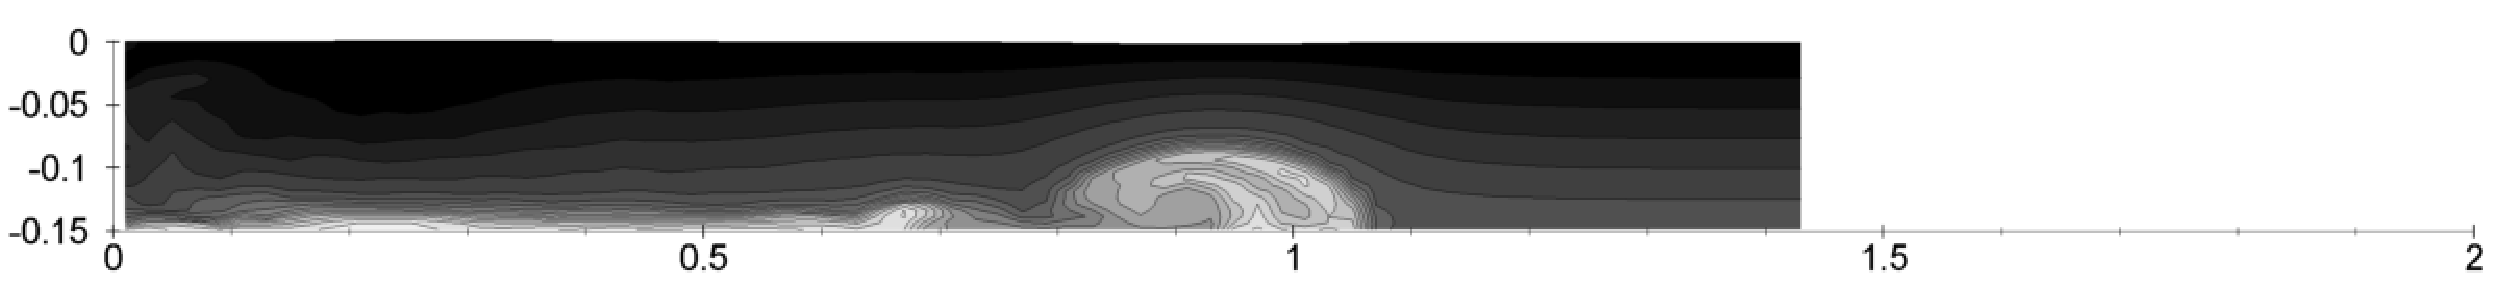
\includegraphics[scale=0.35]{../figures/Exp3-CASE1-dt0.005/rec_2_buf_24_sub_10/D2-102.pdf}    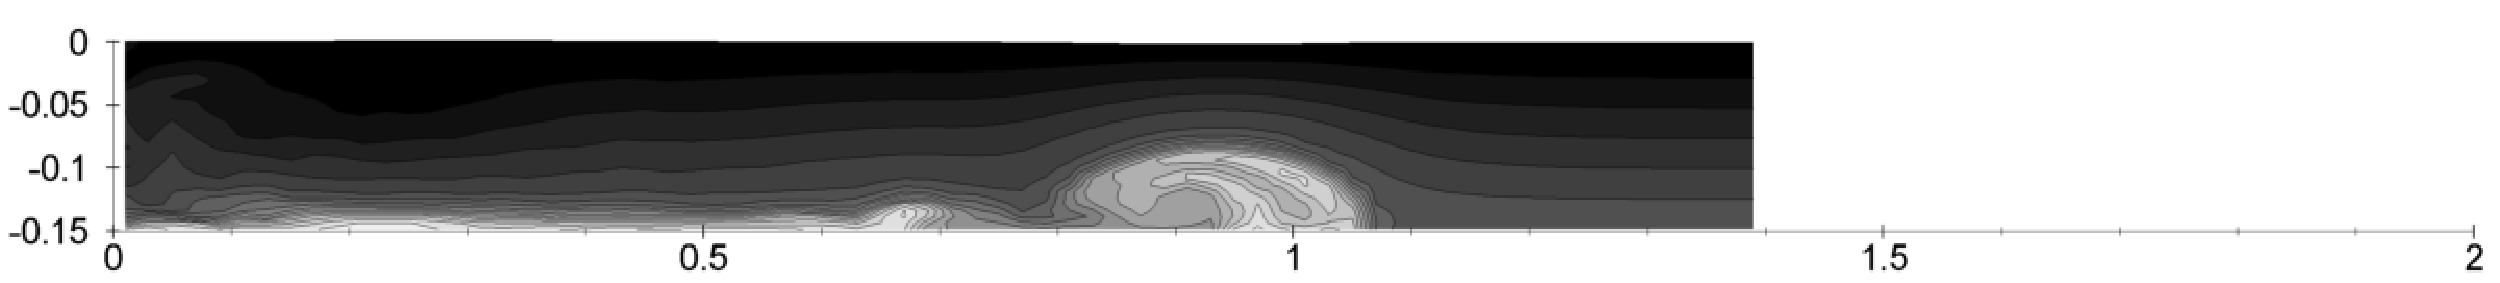
\includegraphics[scale=0.35]{../figures/Exp3-CASE1-dt0.005/rec_2_buf_24_sub_10/D2-103.pdf}
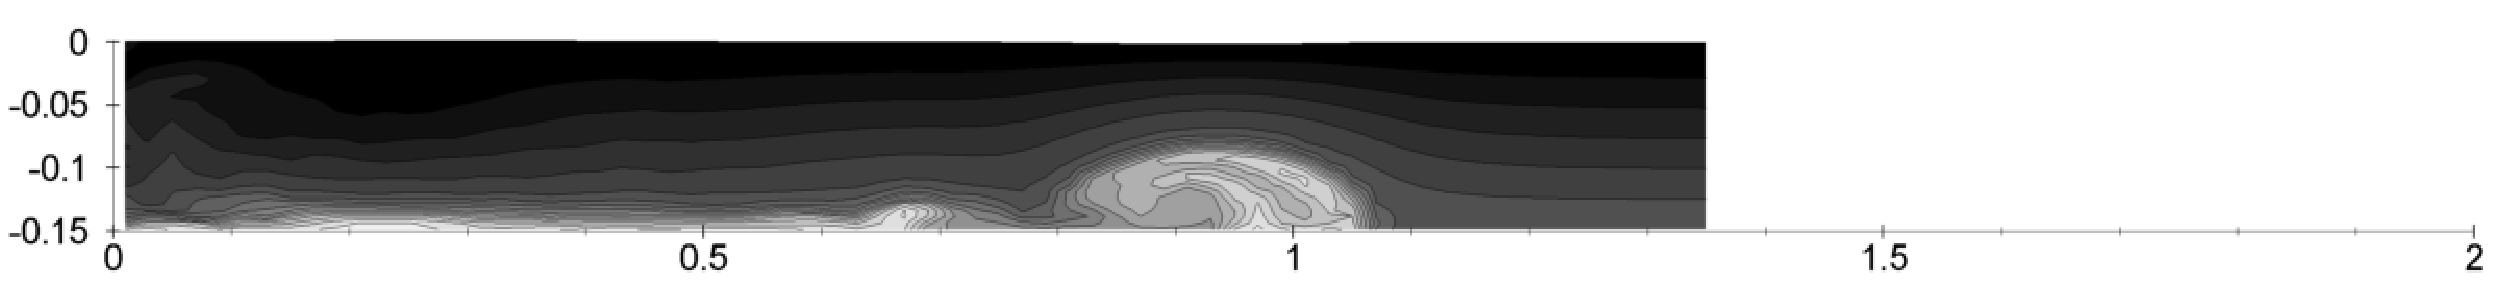
\includegraphics[scale=0.35]{../figures/Exp3-CASE1-dt0.005/rec_2_buf_24_sub_10/D2-104.pdf}    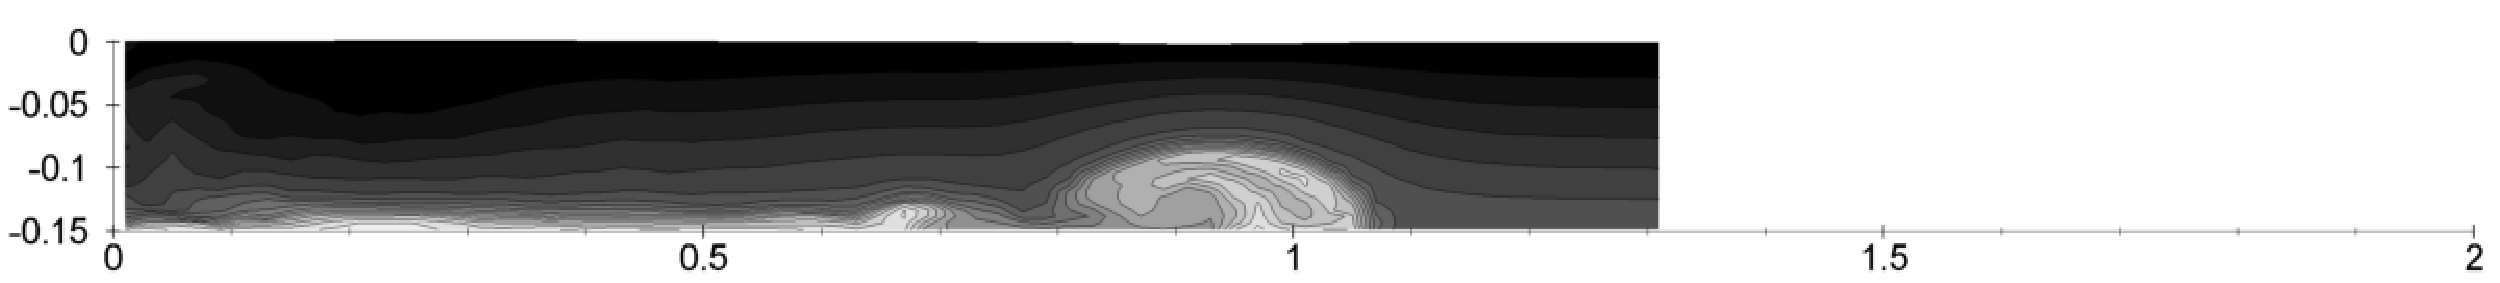
\includegraphics[scale=0.35]{../figures/Exp3-CASE1-dt0.005/rec_2_buf_24_sub_10/D2-105.pdf}
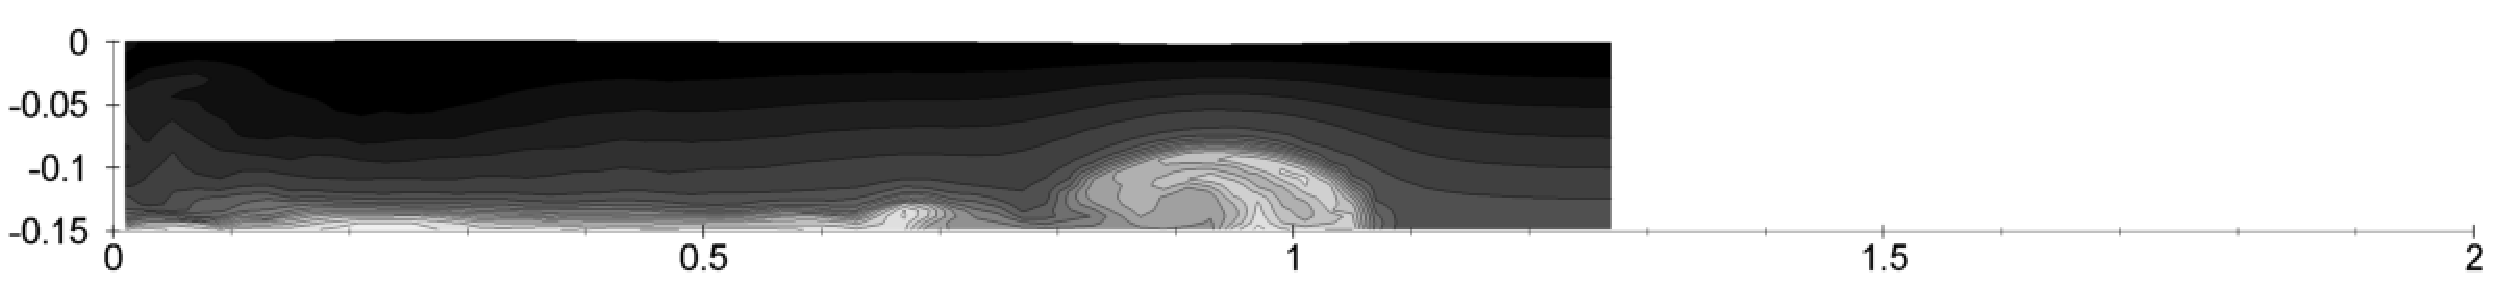
\includegraphics[scale=0.35]{../figures/Exp3-CASE1-dt0.005/rec_2_buf_24_sub_10/D2-106.pdf}    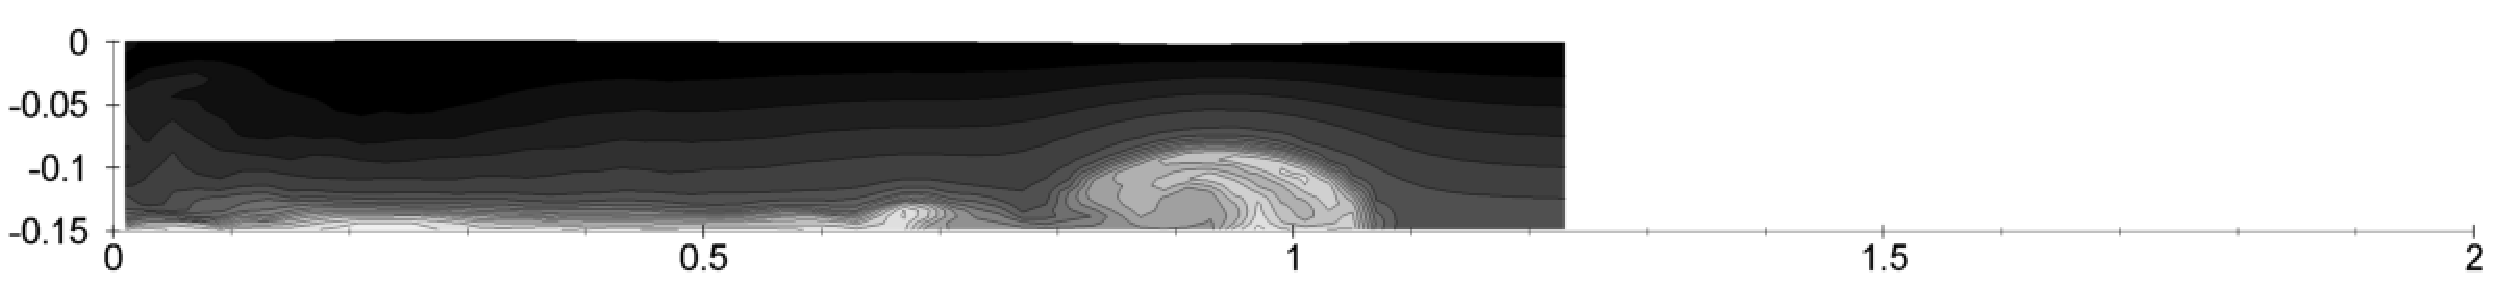
\includegraphics[scale=0.35]{../figures/Exp3-CASE1-dt0.005/rec_2_buf_24_sub_10/D2-107.pdf}
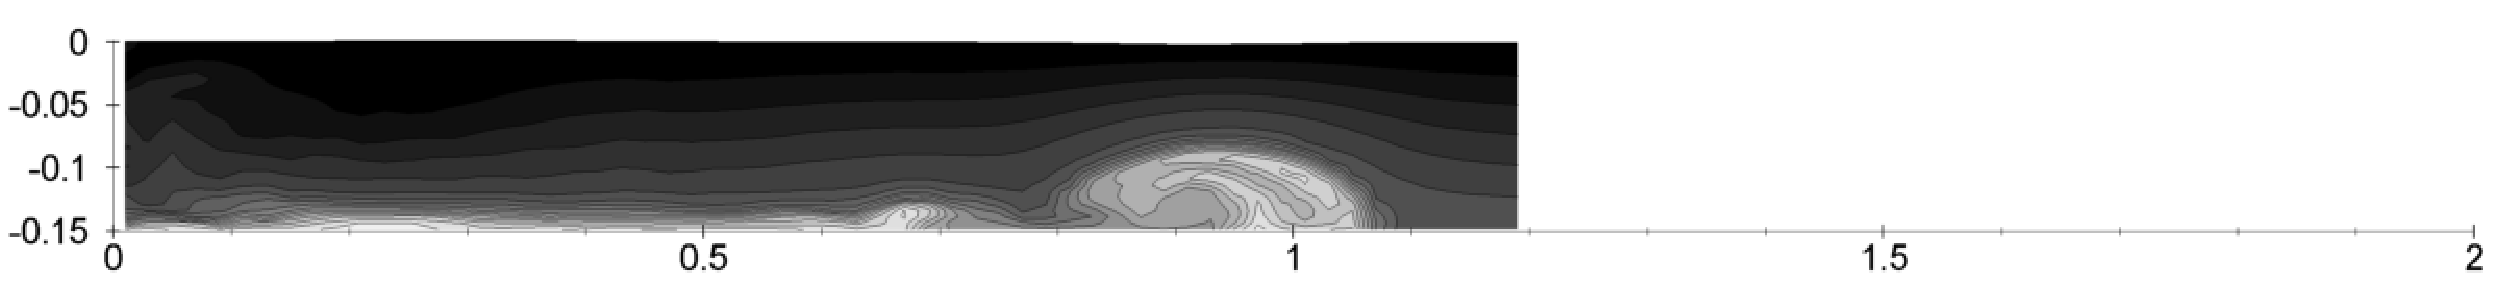
\includegraphics[scale=0.35]{../figures/Exp3-CASE1-dt0.005/rec_2_buf_24_sub_10/D2-108.pdf}    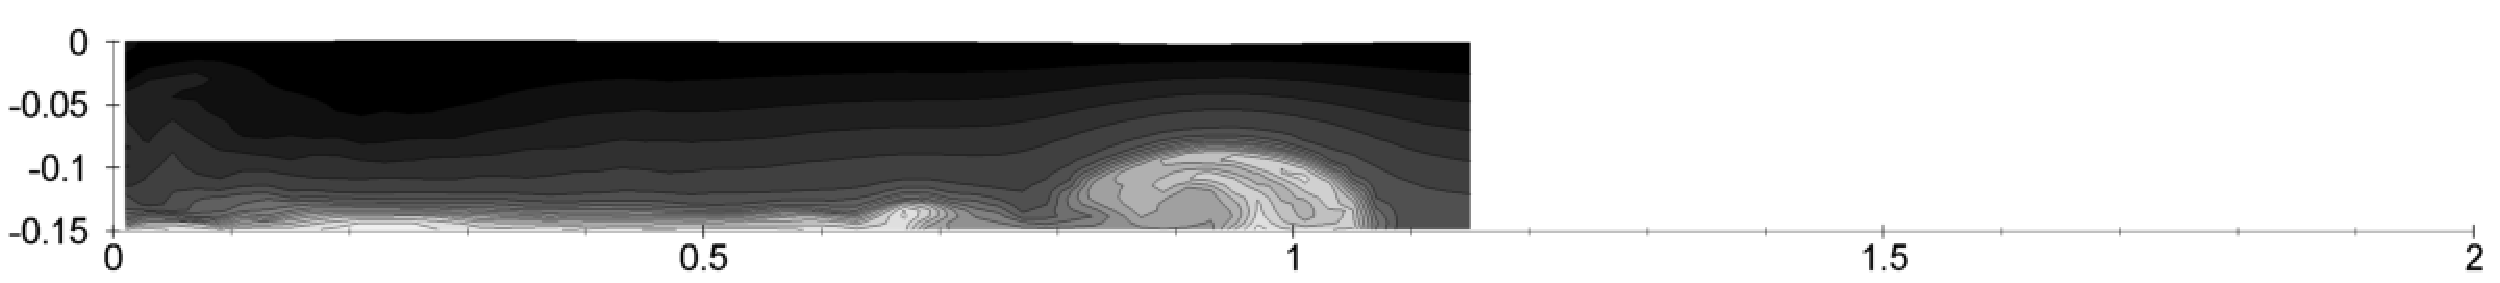
\includegraphics[scale=0.35]{../figures/Exp3-CASE1-dt0.005/rec_2_buf_24_sub_10/D2-109.pdf}
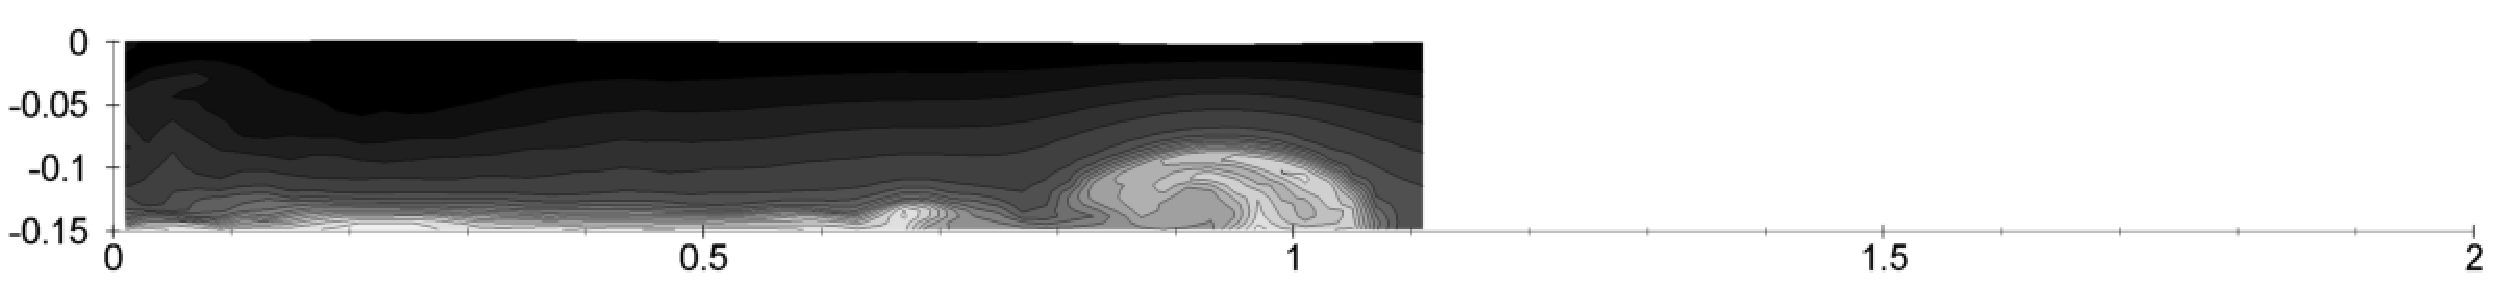
\includegraphics[scale=0.35]{../figures/Exp3-CASE1-dt0.005/rec_2_buf_24_sub_10/D2-110.pdf}
    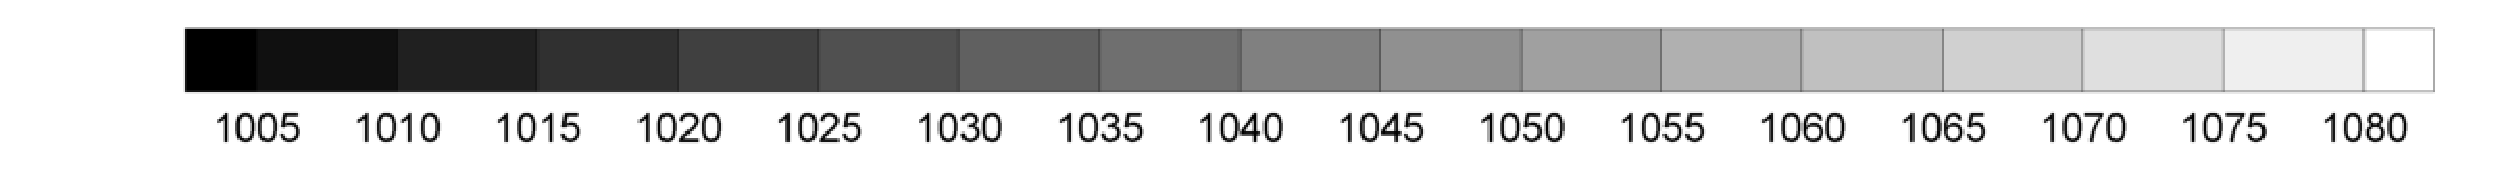
\includegraphics[scale=0.35]{../figures/Exp3-CASE1-dt0.005/legend.pdf}
    \caption{Gravity current simulation with RBM (S=10 B=24 G=2). The figures are the left-hand-side subdomain at $t=6.60-6.65(sec)$}
    \label{fig:RBM-GC-2Domain-L-S10-B24-G2-660}
  \end{center}
\end{figure}

\cp

\begin{figure}[htbp]
  \begin{center}    \includegraphics[scale=0.35]{../figures/Exp3-CASE1-dt0.005/rec_2_buf_24_sub_10/01.pdf}    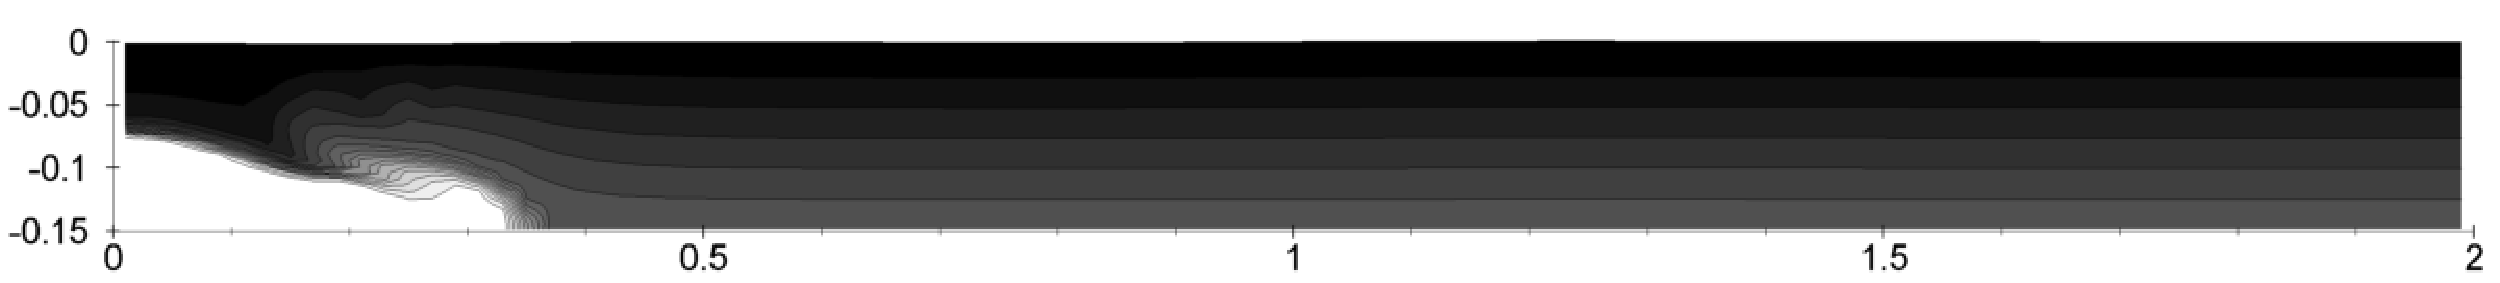
\includegraphics[scale=0.35]{../figures/Exp3-CASE1-dt0.005/rec_2_buf_24_sub_10/03.pdf}
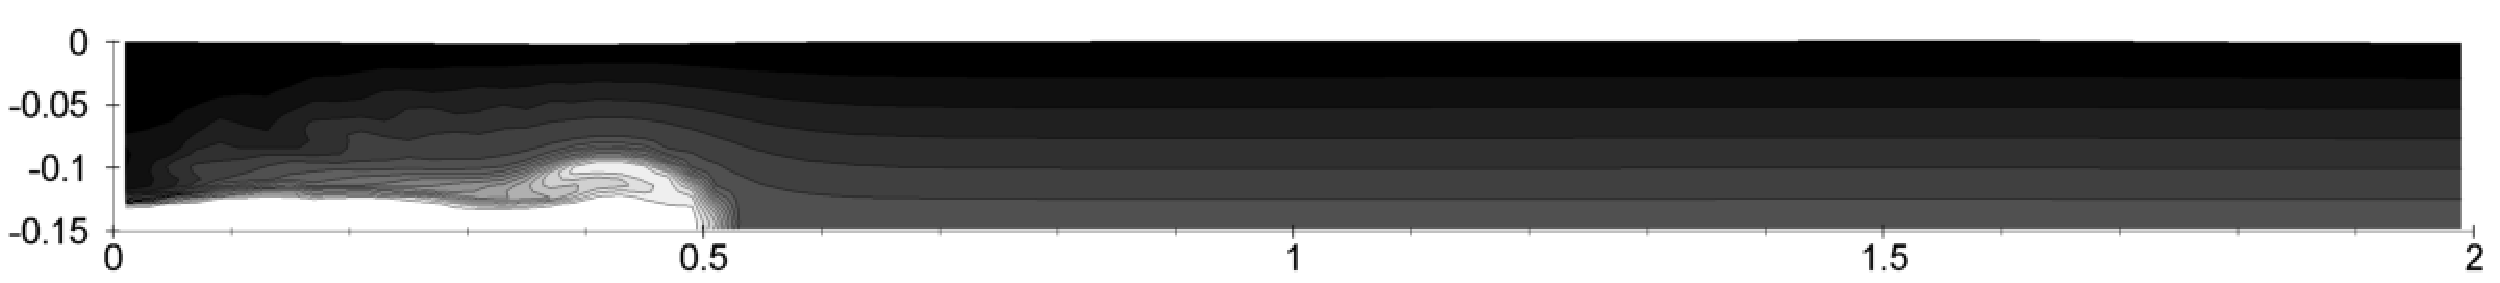
\includegraphics[scale=0.35]{../figures/Exp3-CASE1-dt0.005/rec_2_buf_24_sub_10/05.pdf}
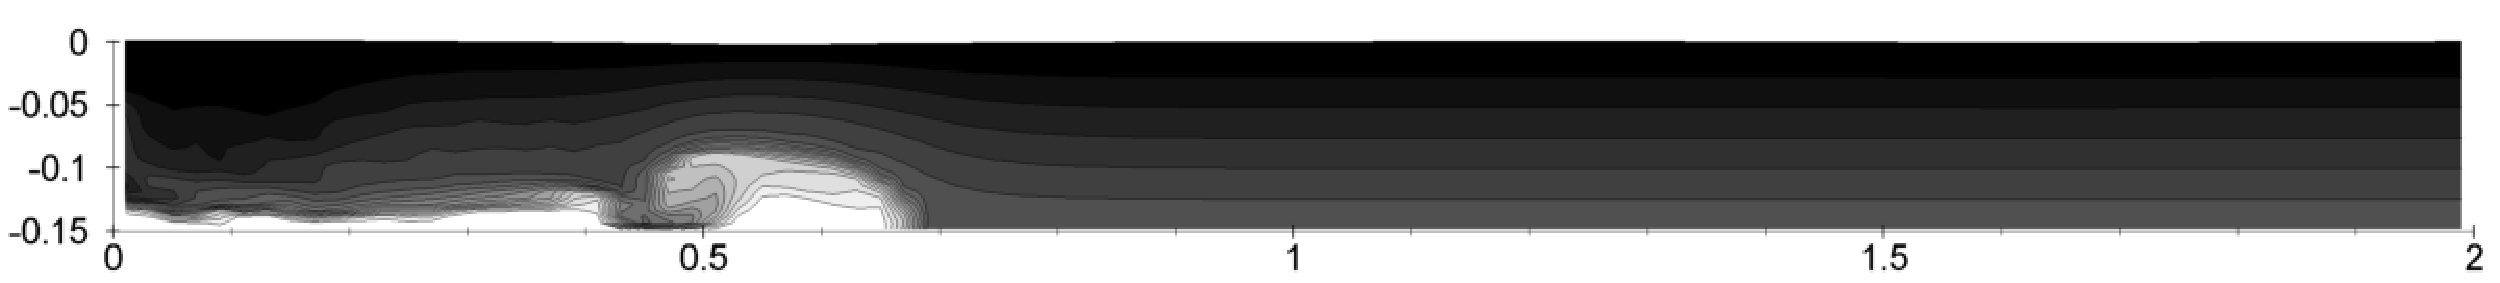
\includegraphics[scale=0.35]{../figures/Exp3-CASE1-dt0.005/rec_2_buf_24_sub_10/07.pdf}    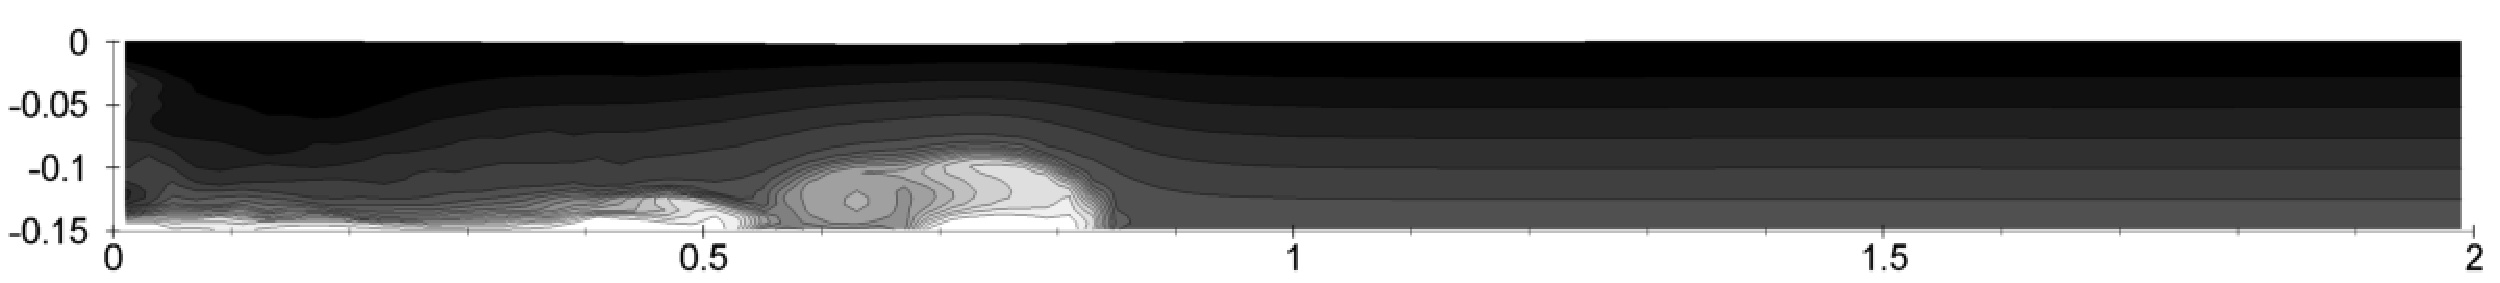
\includegraphics[scale=0.35]{../figures/Exp3-CASE1-dt0.005/rec_2_buf_24_sub_10/09.pdf}
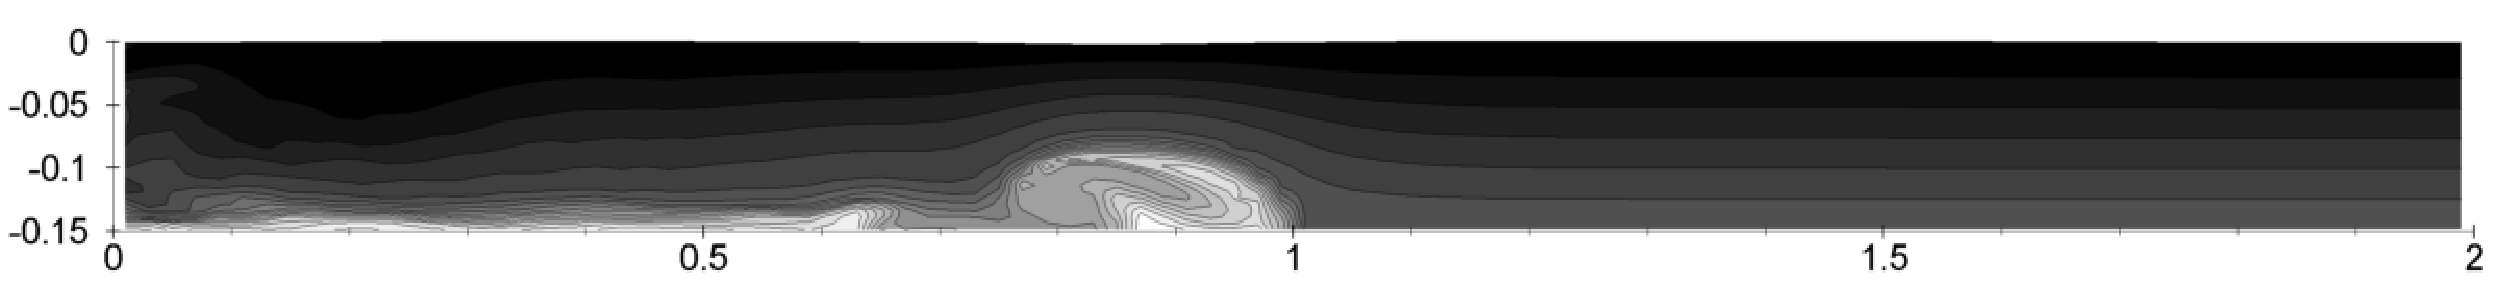
\includegraphics[scale=0.35]{../figures/Exp3-CASE1-dt0.005/rec_2_buf_24_sub_10/11.pdf}
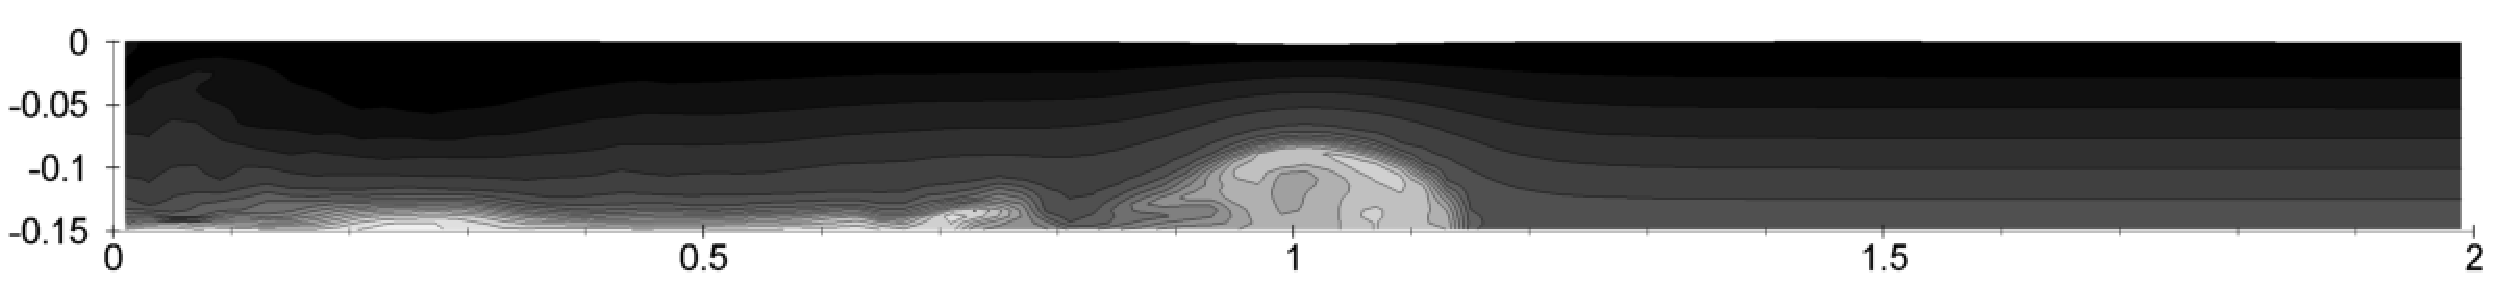
\includegraphics[scale=0.35]{../figures/Exp3-CASE1-dt0.005/rec_2_buf_24_sub_10/13.pdf}    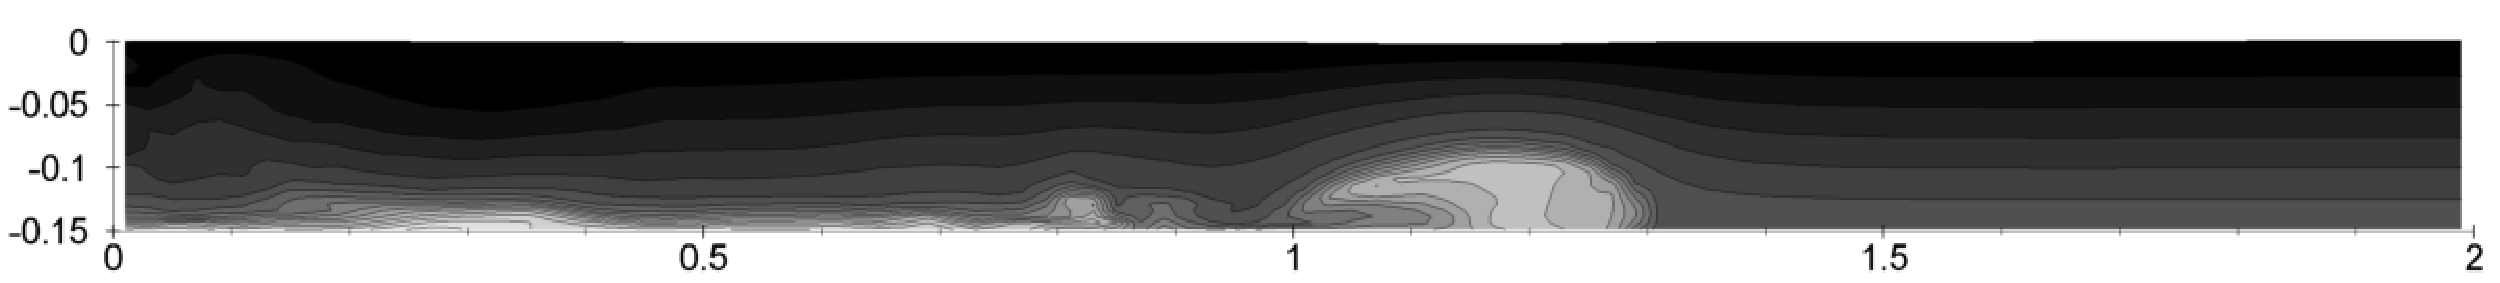
\includegraphics[scale=0.35]{../figures/Exp3-CASE1-dt0.005/rec_2_buf_24_sub_10/15.pdf}
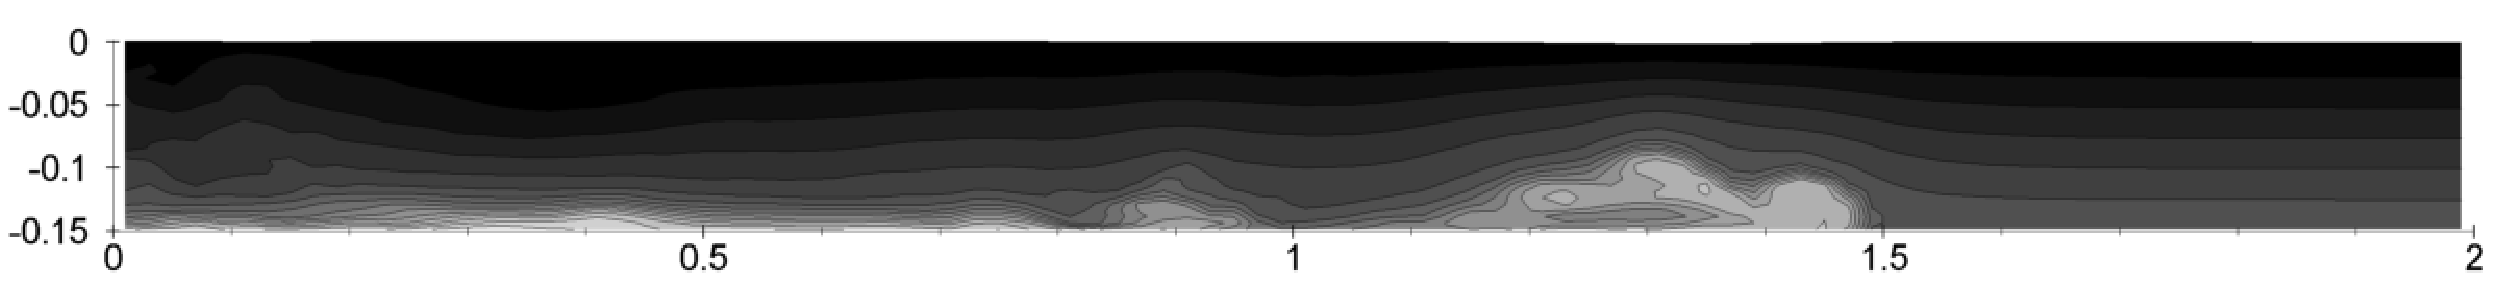
\includegraphics[scale=0.35]{../figures/Exp3-CASE1-dt0.005/rec_2_buf_24_sub_10/17.pdf}    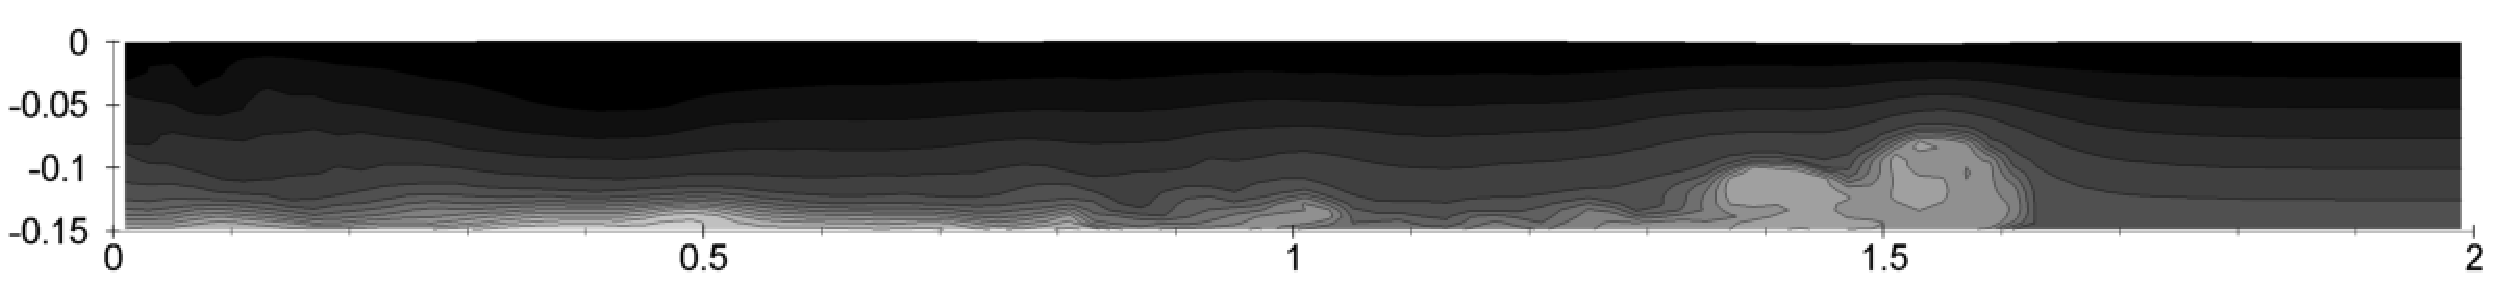
\includegraphics[scale=0.35]{../figures/Exp3-CASE1-dt0.005/rec_2_buf_24_sub_10/19.pdf}
    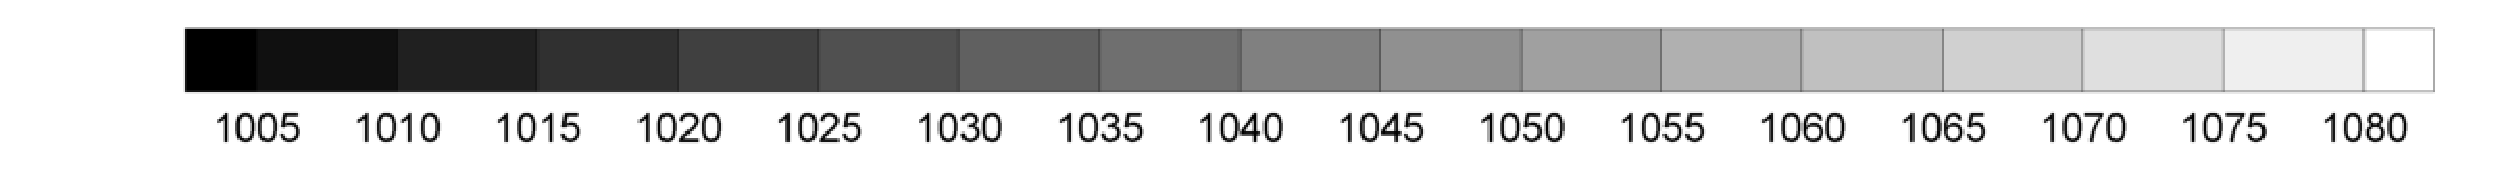
\includegraphics[scale=0.35]{../figures/Exp3-CASE1-dt0.005/legend.pdf}
    \caption{Gravity current simulation with RBM (S=10 B=24 G=2). The figures are merged from the two subdomains}
    \label{fig:RBM-GC-2Domain-S10-B24-G2-660}
  \end{center}
\end{figure}


\cp

\begin{figure}[htbp]
  \begin{center}
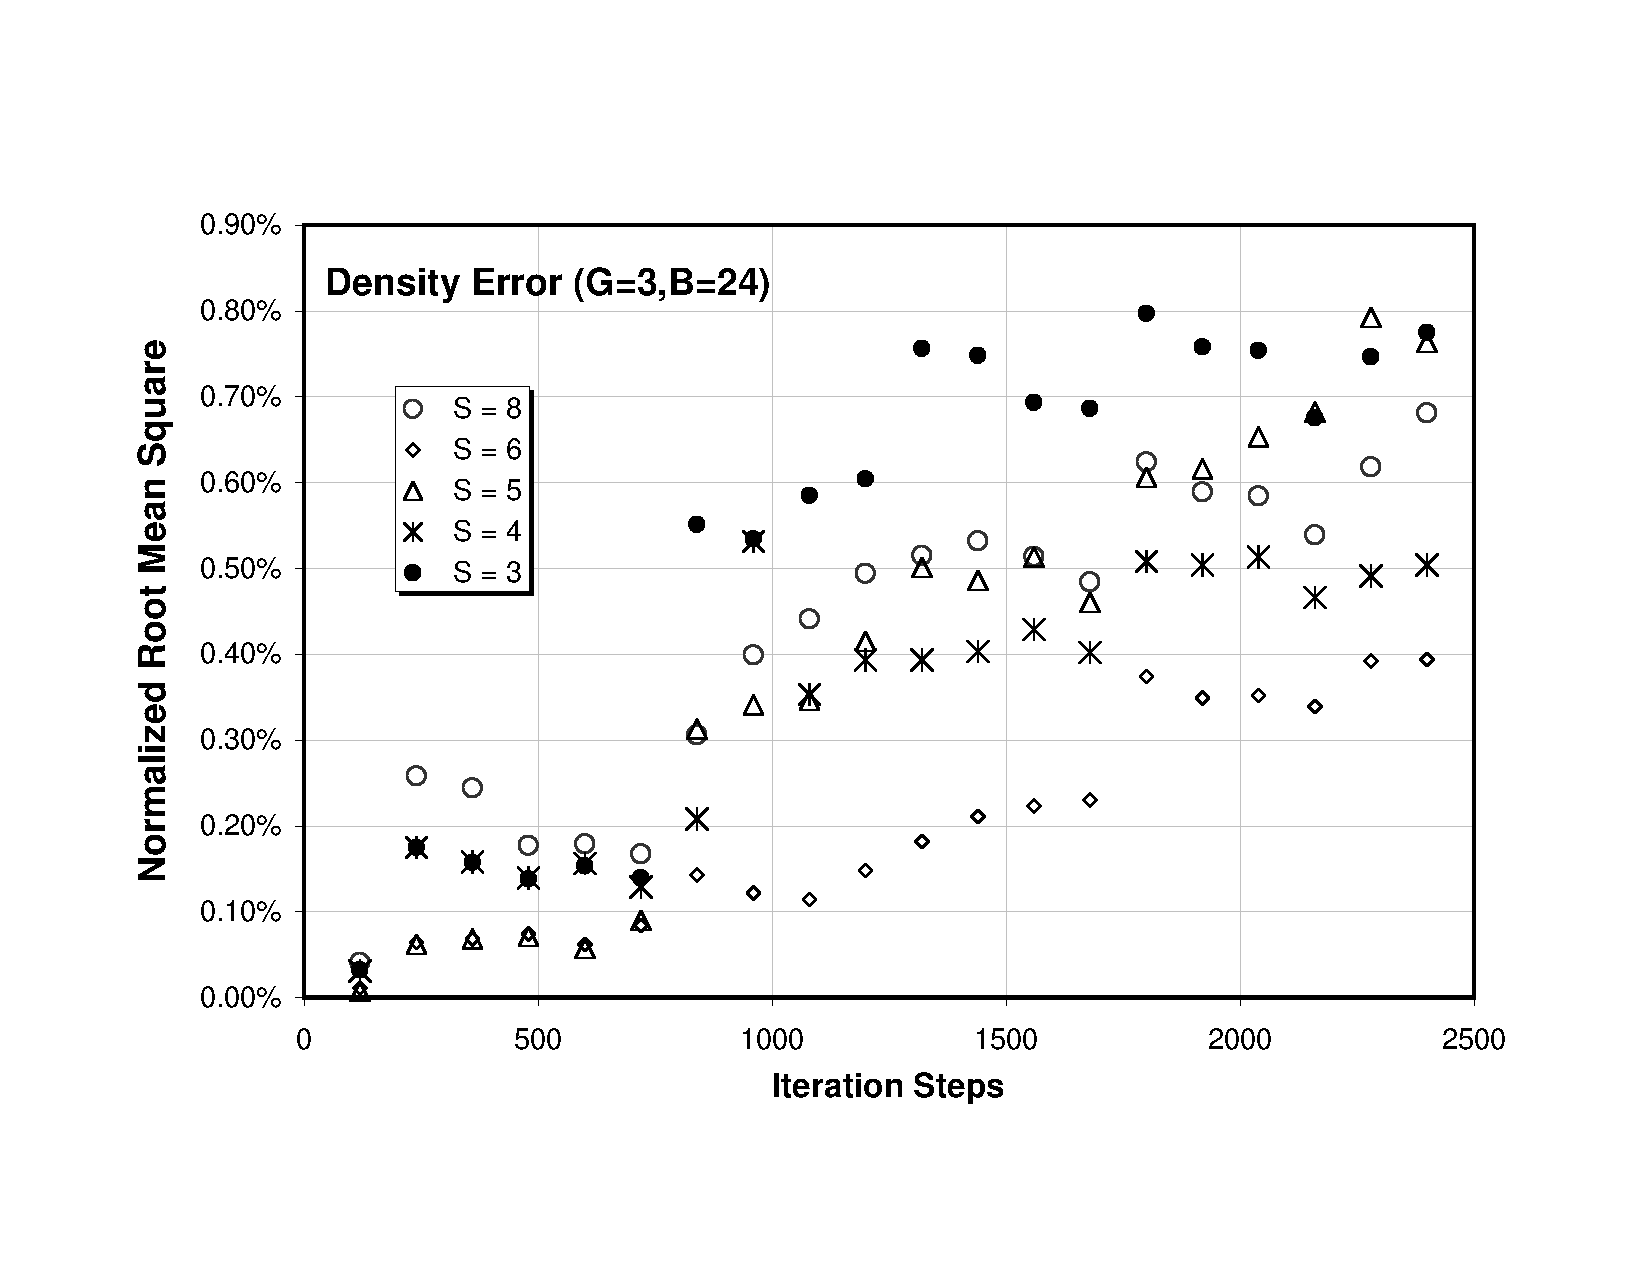
\includegraphics[scale=0.6]{../figures/Exp3-CASE1-dt0.005/G_3_B_24/G3-B24-Den-NRMS.pdf}
    \caption{Density errors(L2) of RBM for the same receding rate (G=3) and buffer (B=24) but different subiterations (S)}
        \vspace{0.5in}
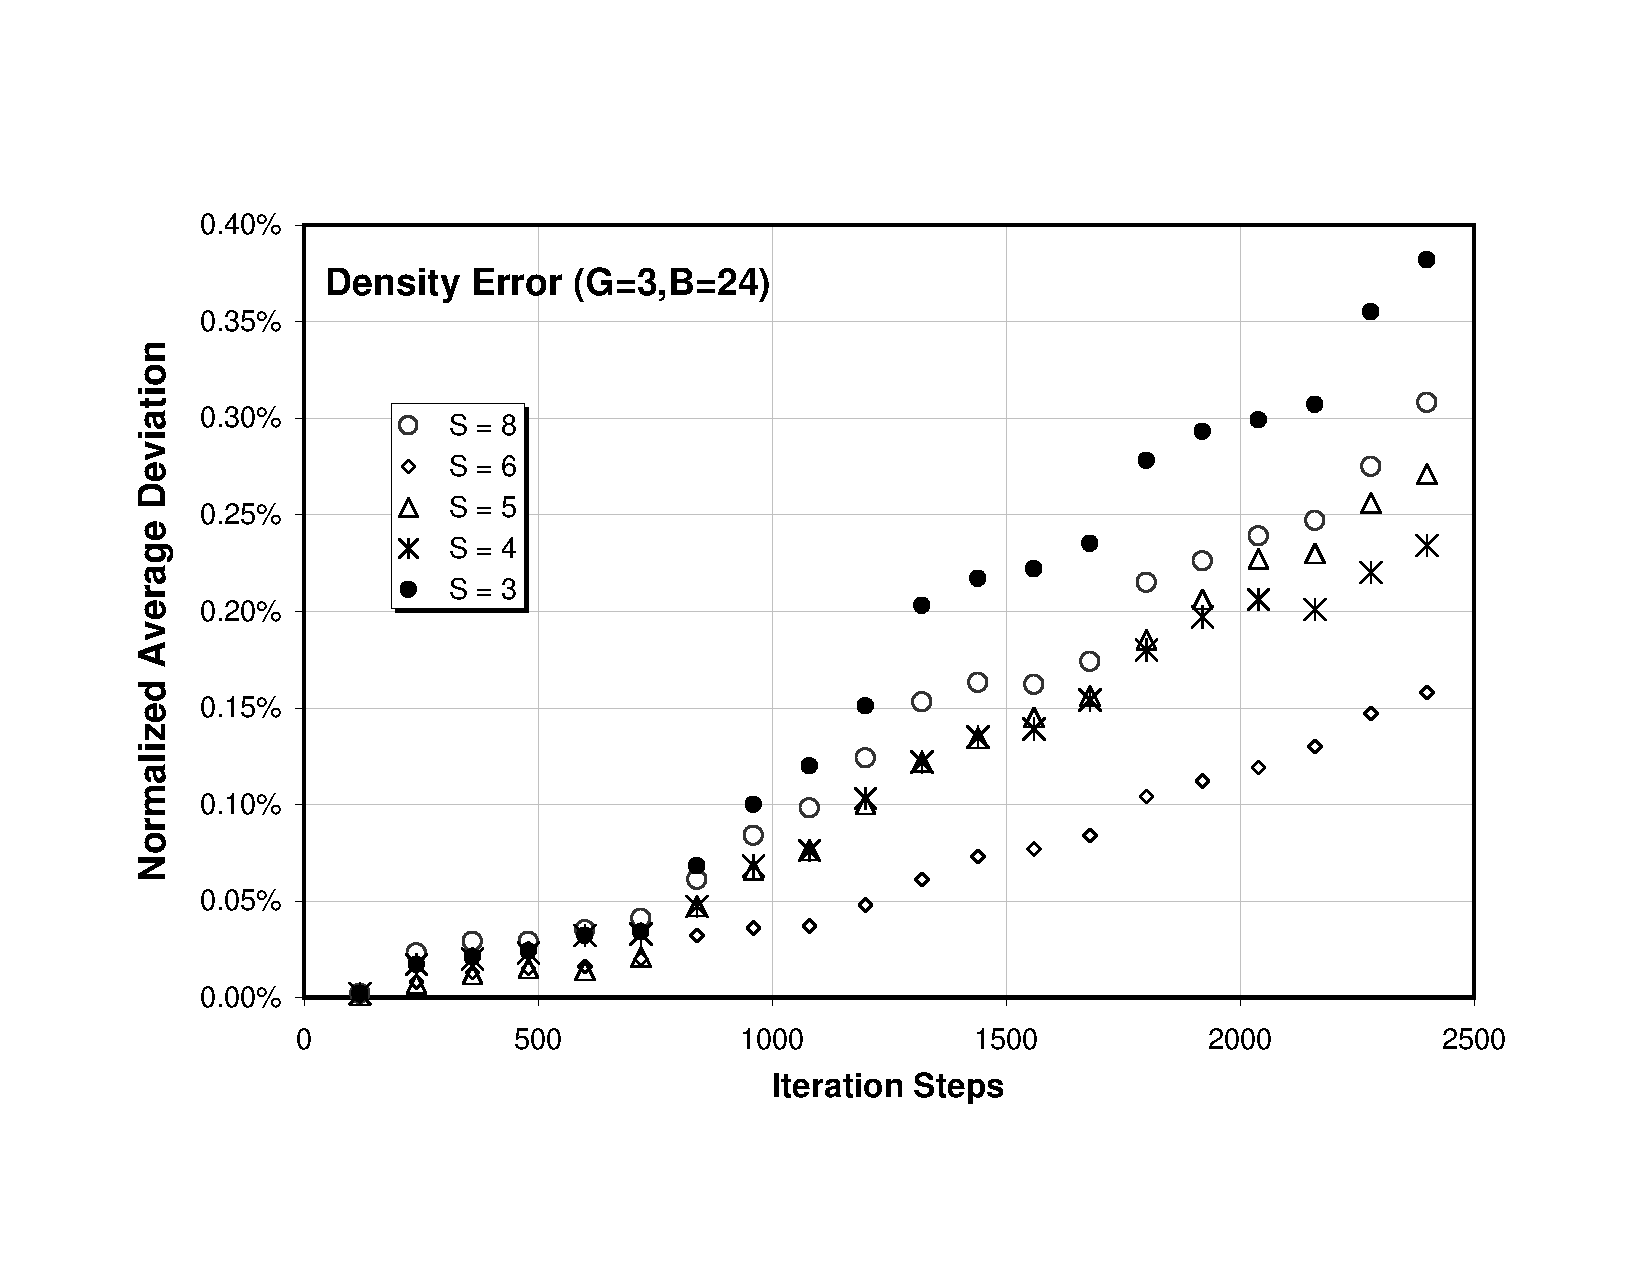
\includegraphics[scale=0.6]{../figures/Exp3-CASE1-dt0.005/G_3_B_24/G3-B24-Den-NAD.pdf}
    \caption{Density errors(L1) of RBM for the same receding rate (G=3) and buffer (B=24) but different subiterations (S)}
  \end{center}
\end{figure}

\cp

\begin{figure}[htbp]
  \begin{center}    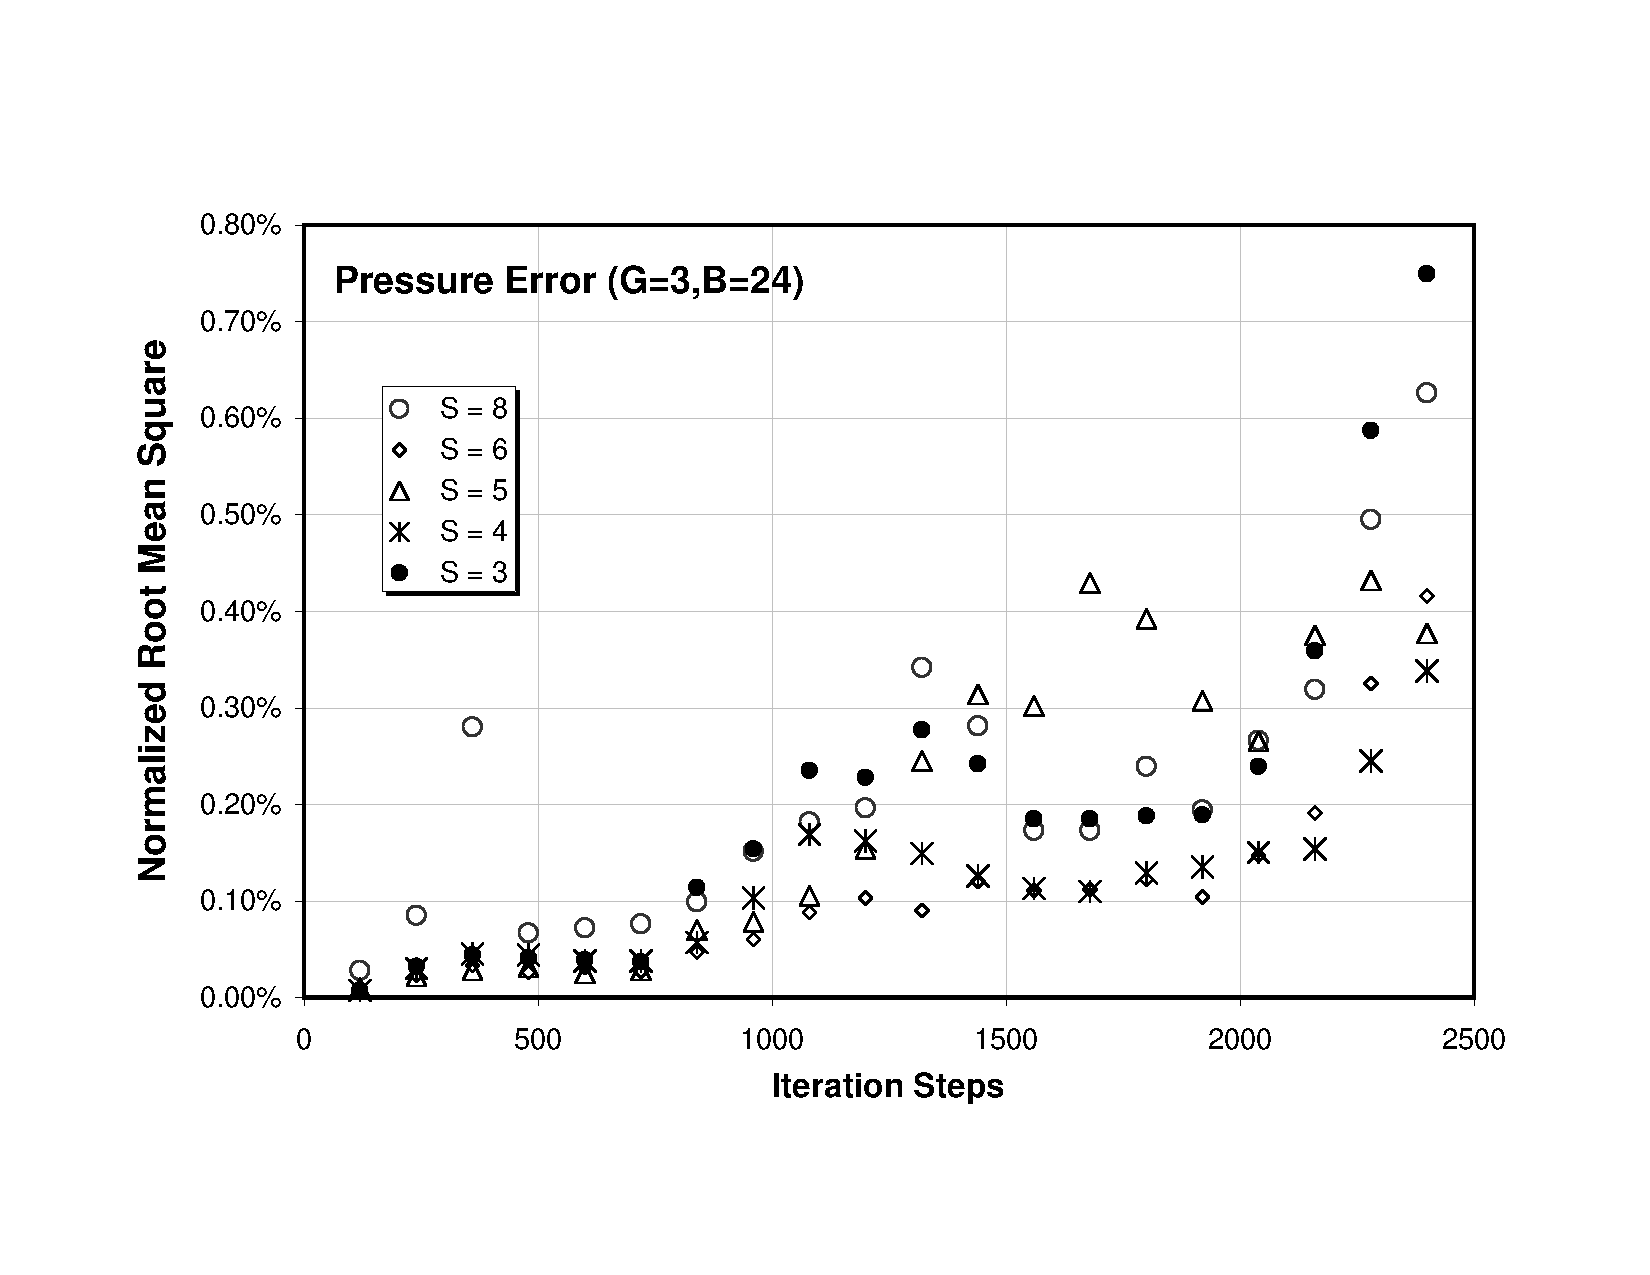
\includegraphics[scale=0.6]{../figures/Exp3-CASE1-dt0.005/G_3_B_24/G3-B24-P-NRMS.pdf}
    \caption{Pressure errors(L2) of RBM for the same receding rate (G=3) and buffer (B=24) but different subiterations (S)}
        \vspace{0.5in}        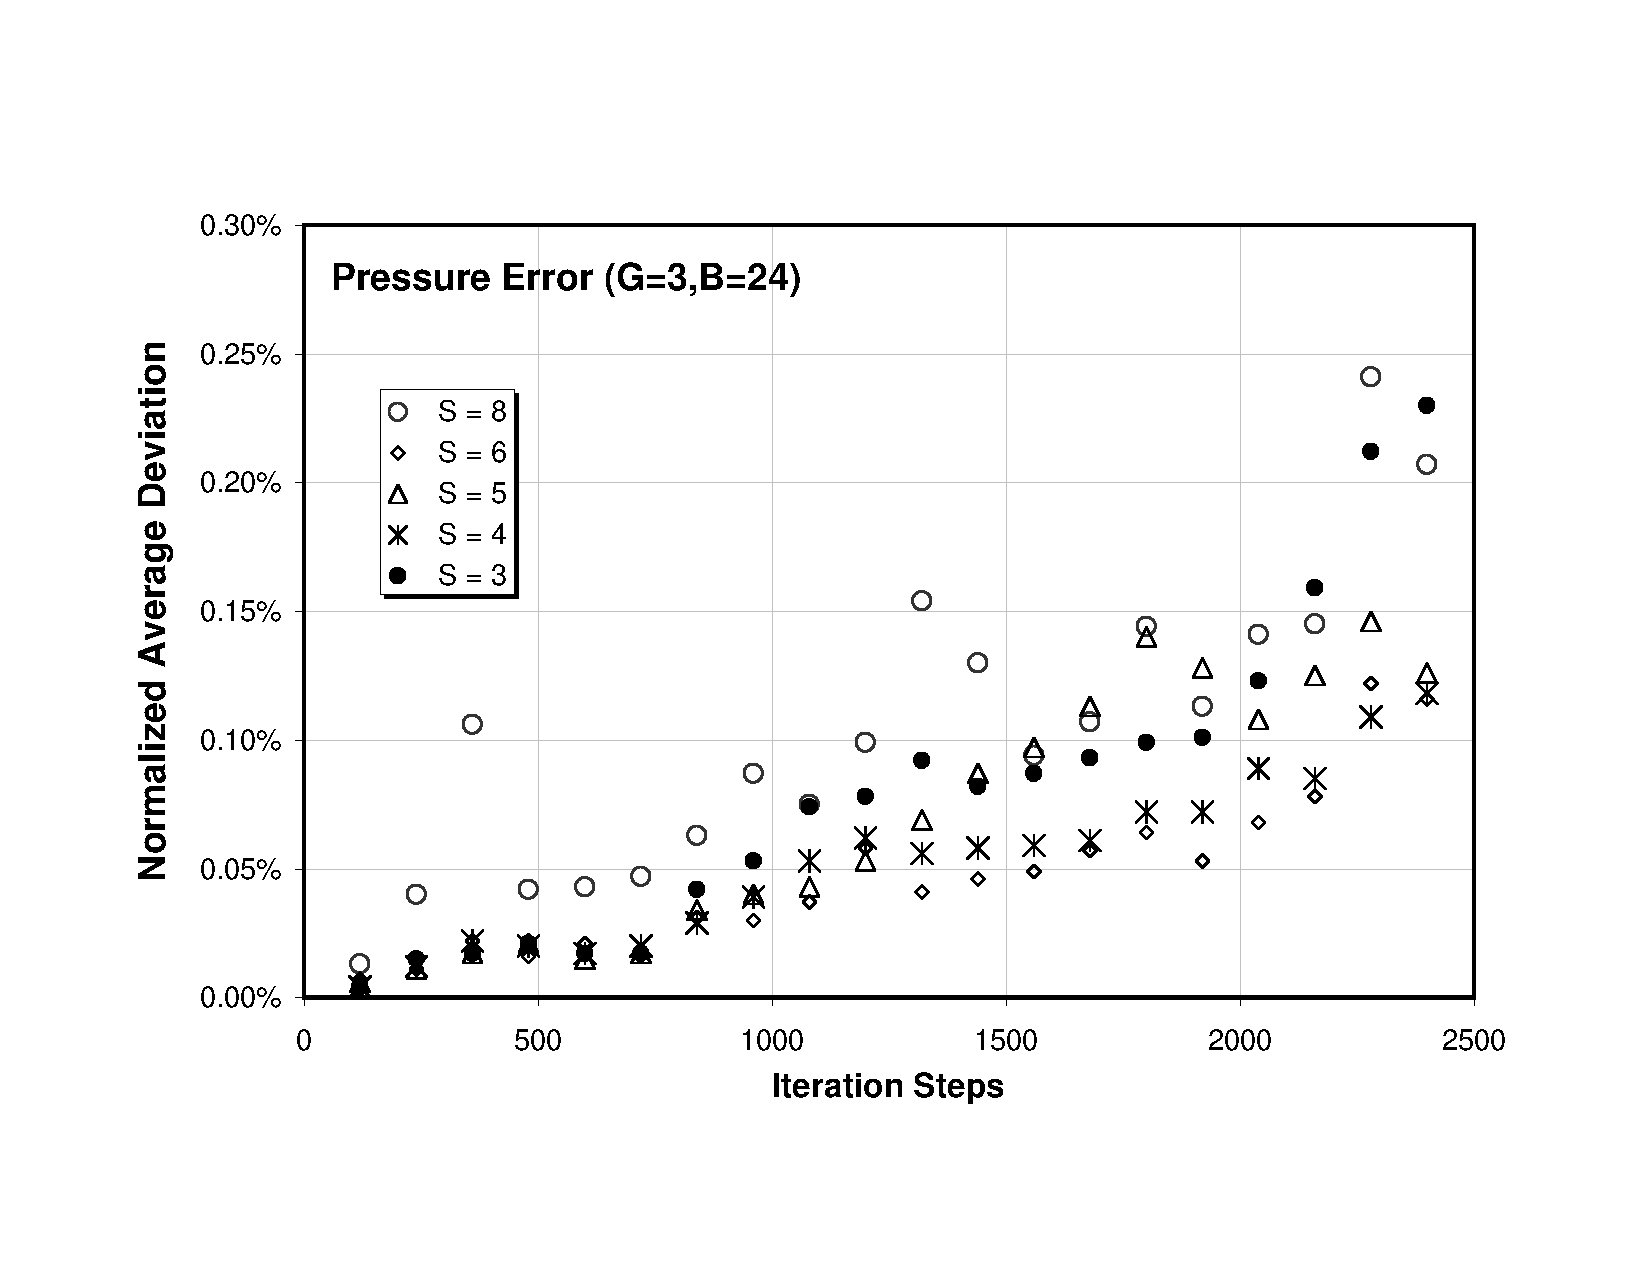
\includegraphics[scale=0.6]{../figures/Exp3-CASE1-dt0.005/G_3_B_24/G3-B24-P-NAD.pdf}
    \caption{Pressure errors(L1) of RBM for the same receding rate (G=3) and buffer (B=24) but different subiterations (S)}
  \end{center}
\end{figure}

\cp

\begin{figure}[htbp]
  \begin{center}
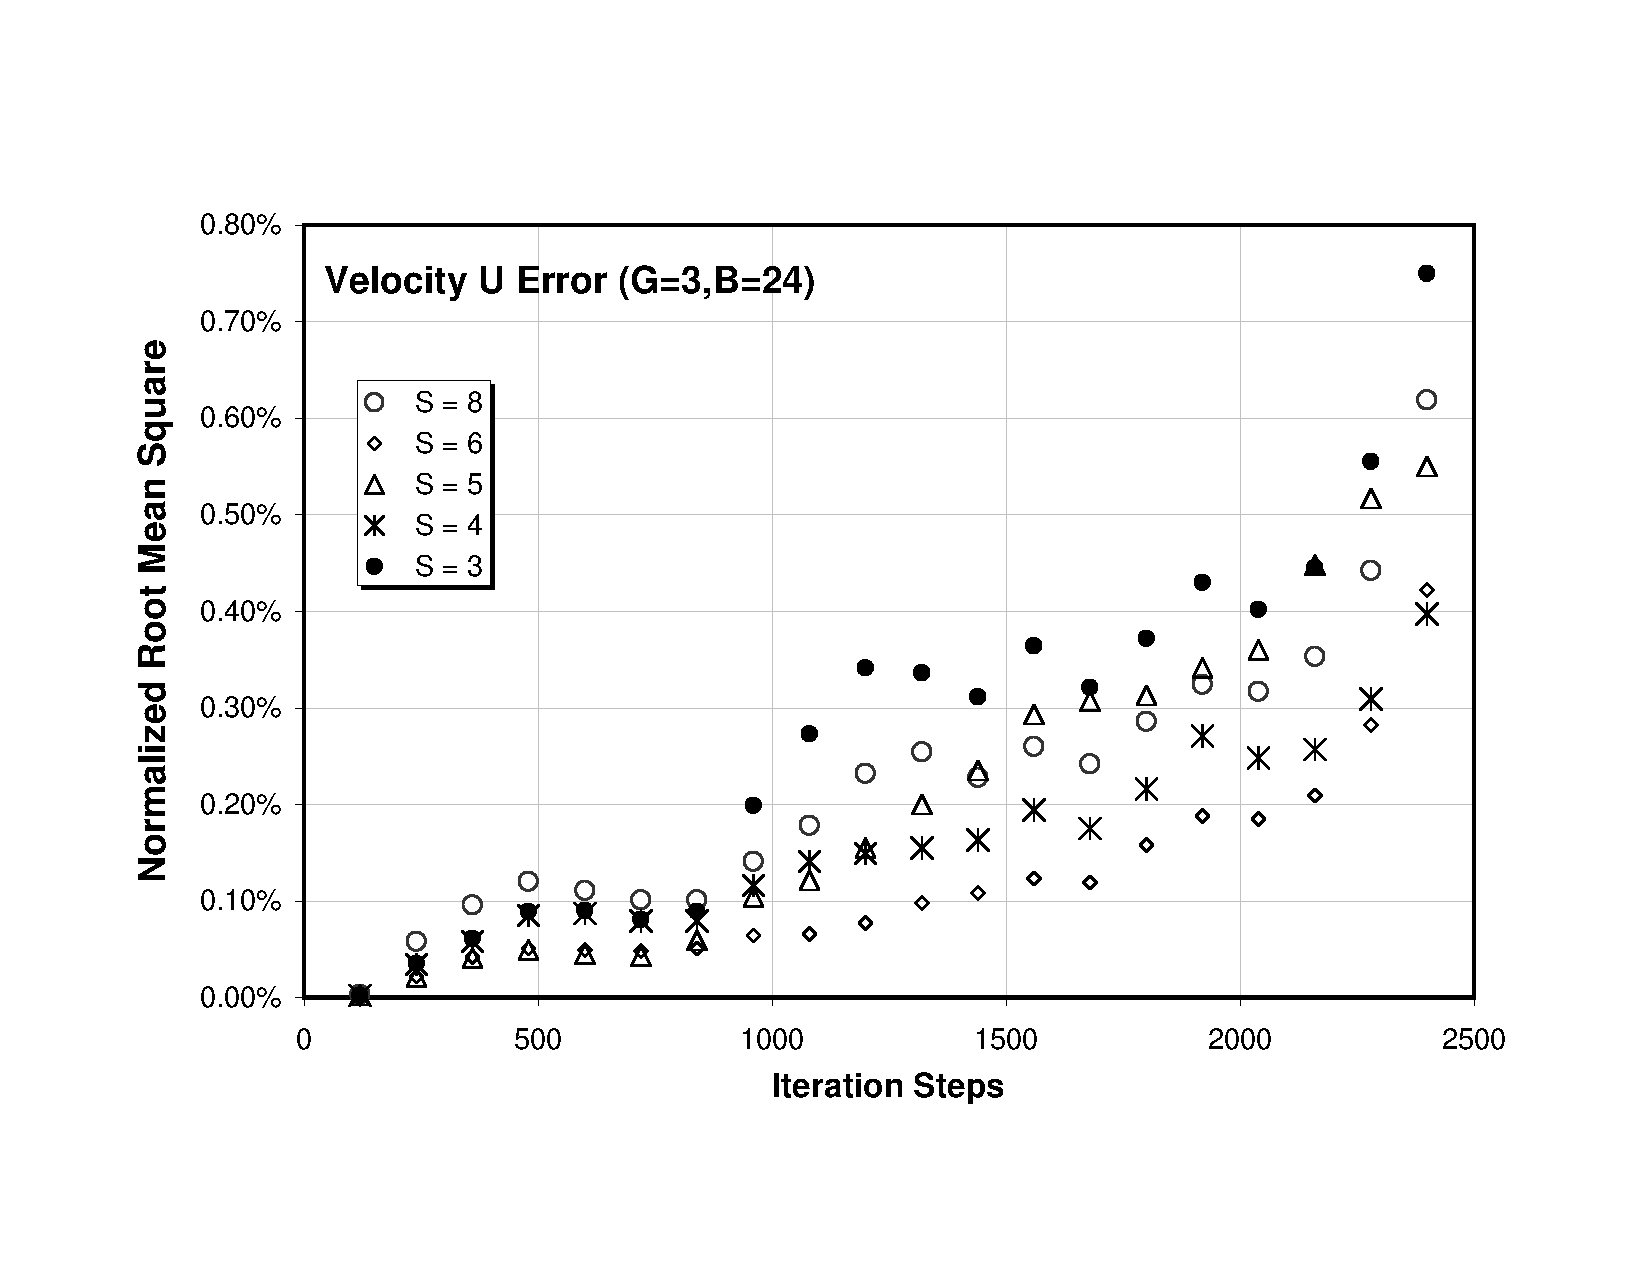
\includegraphics[scale=0.6]{../figures/Exp3-CASE1-dt0.005/G_3_B_24/G3-B24-U-NRMS.pdf}
    \caption{Velocity $u$ errors(L2) of RBM for the same receding rate (G=3) and buffer (B=24) but different subiterations (S)}
    \vspace{0.5in}
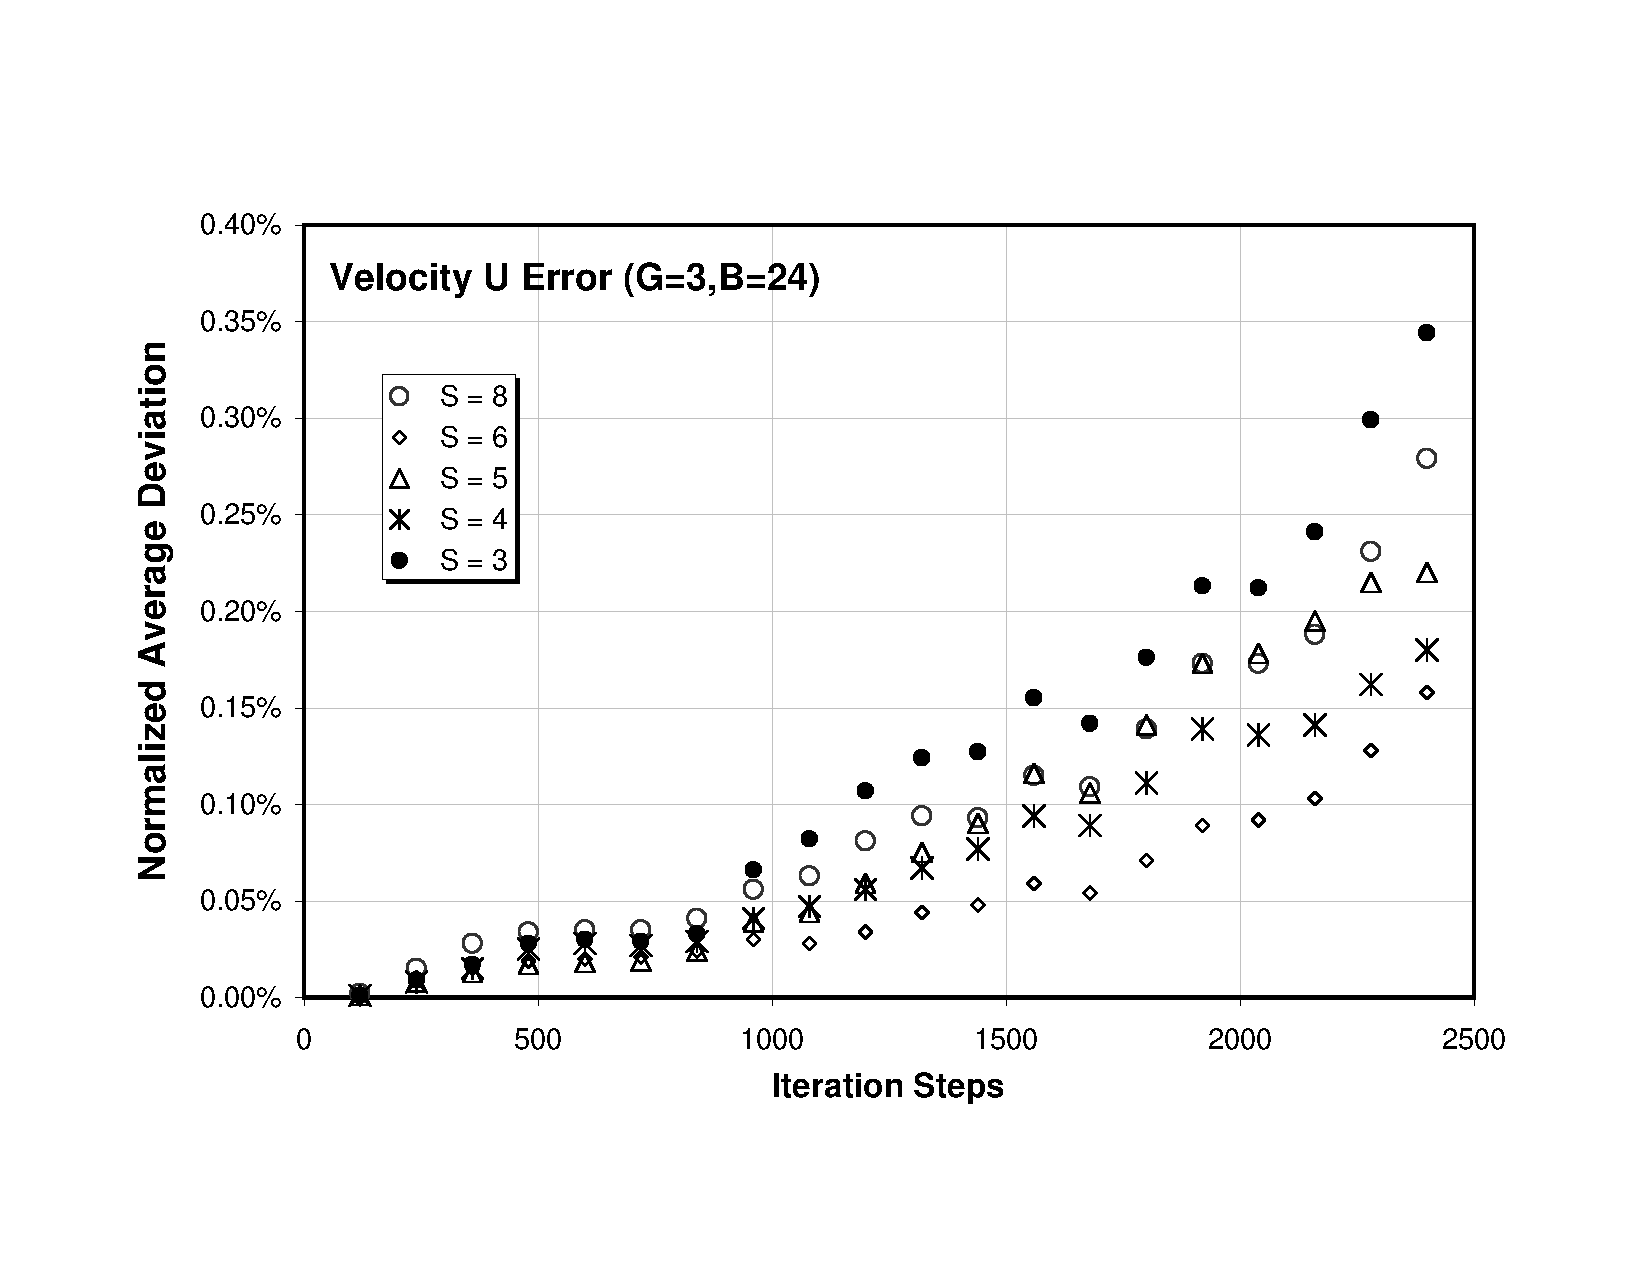
\includegraphics[scale=0.6]{../figures/Exp3-CASE1-dt0.005/G_3_B_24/G3-B24-U-NAD.pdf}
    \caption{Velocity $u$ errors(L1) of RBM for the same receding rate (G=3) and buffer (B=24) but different subiterations (S)}
  \end{center}
\end{figure}

\cp

\begin{figure}[htbp]
  \begin{center}
\includegraphics[scale=0.6]{../figures/Exp3-CASE1-dt0.005/G_3_B_24/G3-B24-W-NRMS.pdf}
    \caption{Velocity $w$ errors(L2) of RBM for the same receding rate (G=3) and buffer (B=24) but different subiterations (S)}
    \vspace{0.5in}
\includegraphics[scale=0.6]{../figures/Exp3-CASE1-dt0.005/G_3_B_24/G3-B24-W-NAD.pdf}
    \caption{Velocity $w$ errors(L1) of RBM for the same receding rate (G=3) and buffer (B=24) but different subiterations (S)}
  \end{center}
\end{figure}


\cp



\begin{figure}[htbp]
  \begin{center}
\includegraphics[scale=0.6]{../figures/Exp3-CASE1-dt0.005/G_2_B_24/G2-B24-Den-NRMS.pdf}
    \caption{Density errors(L2) of RBM for the same receding rate (G=2) and buffer (B=24) but different subiterations (S)}
    \label{fig:RBM-GC-den-error-G2-B24}

        \vspace{0.5in}
\includegraphics[scale=0.6]{../figures/Exp3-CASE1-dt0.005/G_2_B_24/G2-B24-Den-NAD.pdf}
    \caption{Density errors(L1) of RBM for the same receding rate (G=2) and buffer (B=24) but different subiterations (S)}
  \end{center}
\end{figure}

\cp

\begin{figure}[htbp]
  \begin{center}    \includegraphics[scale=0.6]{../figures/Exp3-CASE1-dt0.005/G_2_B_24/G2-B24-P-NRMS.pdf}
    \caption{Pressure errors(L2) of RBM for the same receding rate (G=2) and buffer (B=24) but different subiterations (S)}
        \vspace{0.5in}
\includegraphics[scale=0.6]{../figures/Exp3-CASE1-dt0.005/G_2_B_24/G2-B24-P-NAD.pdf}
    \caption{Pressure errors(L1) of RBM for the same receding rate (G=2) and buffer (B=24) but different subiterations (S)}
  \end{center}
\end{figure}

\cp

\begin{figure}[htbp]
  \begin{center}
\includegraphics[scale=0.6]{../figures/Exp3-CASE1-dt0.005/G_2_B_24/G2-B24-U-NRMS.pdf}
    \caption{Velocity $u$ errors(L2) of RBM for the same receding rate (G=2) and buffer (B=24) but different subiterations (S)}
        \vspace{0.5in}
\includegraphics[scale=0.6]{../figures/Exp3-CASE1-dt0.005/G_2_B_24/G2-B24-U-NAD.pdf}
    \caption{Velocity $u$ errors(L1) of RBM for the same receding rate (G=2) and buffer (B=24) but different subiterations (S)}
  \end{center}
\end{figure}

\cp

\begin{figure}[htbp]
  \begin{center}
\includegraphics[scale=0.6]{../figures/Exp3-CASE1-dt0.005/G_2_B_24/G2-B24-W-NRMS.pdf}
    \caption{Velocity $w$ errors(L2) of RBM for the same receding rate (G=2) and buffer (B=24) but different subiterations (S)}
        \vspace{0.5in}
\includegraphics[scale=0.6]{../figures/Exp3-CASE1-dt0.005/G_2_B_24/G2-B24-W-NAD.pdf}
    \caption{Velocity $w$ errors(L2) of RBM for the same receding rate (G=2) and buffer (B=24) but different subiterations (S)}
  \end{center}
\end{figure}

\cp

\begin{figure}[htbp]
  \begin{center}
\includegraphics[scale=0.6]{../figures/Exp3-CASE1-dt0.005/G_1_B_24/G1-B24-Den-NRMS.pdf}
    \caption{Density errors(L2) of RBM for the same receding rate (G=1) and buffer (B=24) but different subiterations (S)}
        \vspace{0.5in}
\includegraphics[scale=0.6]{../figures/Exp3-CASE1-dt0.005/G_1_B_24/G1-B24-Den-NAD.pdf}
    \caption{Density errors(L1) of RBM for the same receding rate (G=1) and buffer (B=24) but different subiterations (S)}
  \end{center}
\end{figure}

\cp

\begin{figure}[htbp]
  \begin{center}    \includegraphics[scale=0.6]{../figures/Exp3-CASE1-dt0.005/G_1_B_24/G1-B24-P-NRMS.pdf}
    \caption{Pressure errors(L2) of RBM for the same receding rate (G=1) and buffer (B=24) but different subiterations (S)}
        \vspace{0.5in}
\includegraphics[scale=0.6]{../figures/Exp3-CASE1-dt0.005/G_1_B_24/G1-B24-P-NAD.pdf}
    \caption{Pressure errors(L1) of RBM for the same receding rate (G=1) and buffer (B=24) but different subiterations (S)}
  \end{center}
\end{figure}

\cp

\begin{figure}[htbp]
  \begin{center}
\includegraphics[scale=0.6]{../figures/Exp3-CASE1-dt0.005/G_1_B_24/G1-B24-U-NRMS.pdf}
    \caption{Velocity $u$ errors(L2) of RBM for the same receding rate (G=1) and buffer (B=24) but different subiterations (S)}
        \vspace{0.5in}
\includegraphics[scale=0.6]{../figures/Exp3-CASE1-dt0.005/G_1_B_24/G1-B24-U-NAD.pdf}
    \caption{Velocity $u$ errors(L1) of RBM for the same receding rate (G=1) and buffer (B=24) but different subiterations (S)}
  \end{center}
\end{figure}

\cp

\begin{figure}[htbp]
  \begin{center}
\includegraphics[scale=0.6]{../figures/Exp3-CASE1-dt0.005/G_1_B_24/G1-B24-W-NRMS.pdf}
    \caption{Velocity $w$ errors(L2) of RBM for the same receding rate (G=1) and buffer (B=24) but different subiterations (S)}
        \vspace{0.5in}
\includegraphics[scale=0.6]{../figures/Exp3-CASE1-dt0.005/G_1_B_24/G1-B24-W-NAD.pdf}
    \caption{Velocity $w$ errors(L2) of RBM for the same receding rate (G=1) and buffer (B=24) but different subiterations (S)}
  \end{center}
\end{figure}

\cp


\begin{table}[hbtp]%[hbtp]
\vspace{0.6in}
\begin{center}
\caption{Density errors of RBM for the receding rate $G=2$, buffer $B=24$, and subiteration $S=10$} %dt= 0.005
\small
 \begin{tabular}{cccccccc} \hline %{|c|l|r|r|}
 time & step & $error_{2}$ & $error_{1}$ &  min & max &  $error_{2}^*$ & $error_{1}^*$ \\ \hline
  0.6 &   120 & 0.964E-01 & 0.434E-02 & 0.100E+04 & 0.108E+04 &   0.114\% &   0.005\%  \\
  1.2 &   240 & 0.776E-01 & 0.890E-02 & 0.100E+04 & 0.108E+04 &   0.091\% &   0.010\%  \\
  1.8 &   360 & 0.482E-01 & 0.913E-02 & 0.100E+04 & 0.108E+04 &   0.057\% &   0.011\%  \\
  2.4 &   480 & 0.560E-01 & 0.119E-01 & 0.100E+04 & 0.108E+04 &   0.066\% &   0.014\%  \\
  3.0 &   600 & 0.639E-01 & 0.159E-01 & 0.100E+04 & 0.108E+04 &   0.075\% &   0.019\%  \\
  3.6 &   720 & 0.769E-01 & 0.198E-01 & 0.100E+04 & 0.108E+04 &   0.091\% &   0.023\%  \\
  4.2 &   840 & 0.132E+00 & 0.268E-01 & 0.100E+04 & 0.108E+04 &   0.156\% &   0.032\%  \\
  4.8 &   960 & 0.106E+00 & 0.270E-01 & 0.100E+04 & 0.108E+04 &   0.125\% &   0.032\%  \\
  5.4 &  1080 & 0.936E-01 & 0.267E-01 & 0.100E+04 & 0.108E+04 &   0.110\% &   0.031\%  \\
  6.0 &  1200 & 0.956E-01 & 0.312E-01 & 0.100E+04 & 0.108E+04 &   0.115\% &   0.037\%  \\
  6.6 &  1320 & 0.123E+00 & 0.384E-01 & 0.100E+04 & 0.108E+04 &   0.154\% &   0.048\%  \\
  7.2 &  1440 & 0.146E+00 & 0.425E-01 & 0.100E+04 & 0.108E+04 &   0.187\% &   0.054\%  \\
  7.8 &  1560 & 0.180E+00 & 0.511E-01 & 0.100E+04 & 0.108E+04 &   0.232\% &   0.066\%  \\
  8.4 &  1680 & 0.176E+00 & 0.580E-01 & 0.100E+04 & 0.108E+04 &   0.231\% &   0.076\%  \\
  9.0 &  1800 & 0.283E+00 & 0.721E-01 & 0.100E+04 & 0.108E+04 &   0.377\% &   0.096\%  \\
  9.6 &  1920 & 0.266E+00 & 0.811E-01 & 0.100E+04 & 0.107E+04 &   0.364\% &   0.111\%  \\
 10.2 &  2040 & 0.253E+00 & 0.901E-01 & 0.100E+04 & 0.107E+04 &   0.356\% &   0.127\%  \\
 10.8 &  2160 & 0.241E+00 & 0.885E-01 & 0.100E+04 & 0.107E+04 &   0.348\% &   0.128\%  \\
 11.4 &  2280 & 0.253E+00 & 0.887E-01 & 0.100E+04 & 0.107E+04 &   0.374\% &   0.131\%  \\
 12.0 &  2400 & 0.253E+00 & 0.892E-01 & 0.100E+04 & 0.107E+04 &   0.382\% &   0.135\%  \\
 \hline
 \end{tabular}
 \label{tab:1}
 \end{center}
 \end{table}

\cp

 \begin{table}[hbtp]%[hbtp]
\vspace{0.6in}
 \begin{center}
\caption{Pressure errors of RBM for the receding rate $G=2$, buffer $B=24$, and subiteration $S=10$} %dt= 0.005
\small
 \begin{tabular}{cccccccc} \hline %{|c|l|r|r|}
 time & step & $error_{2}$ & $error_{1}$ &  min & max &  $error_{2}^*$ & $error_{1}^*$ \\ \hline
  0.6 &   120 & 0.239E-01 & 0.115E-01 & -.409E+01 & 0.827E+02 &   0.027\% &   0.013\%  \\
  1.2 &   240 & 0.287E-01 & 0.150E-01 & -.789E+00 & 0.697E+02 &   0.041\% &   0.021\%  \\
  1.8 &   360 & 0.140E+00 & 0.488E-01 & -.350E+01 & 0.517E+02 &   0.267\% &   0.093\%  \\
  2.4 &   480 & 0.216E-01 & 0.146E-01 & -.518E+00 & 0.510E+02 &   0.042\% &   0.028\%  \\
  3.0 &   600 & 0.267E-01 & 0.164E-01 & -.386E+00 & 0.534E+02 &   0.050\% &   0.031\%  \\
  3.6 &   720 & 0.247E-01 & 0.160E-01 & -.572E+00 & 0.541E+02 &   0.045\% &   0.029\%  \\
  4.2 &   840 & 0.307E-01 & 0.214E-01 & -.690E+00 & 0.500E+02 &   0.061\% &   0.042\%  \\
  4.8 &   960 & 0.450E-01 & 0.283E-01 & -.380E+00 & 0.497E+02 &   0.090\% &   0.056\%  \\
  5.4 &  1080 & 0.310E-01 & 0.185E-01 & -.566E+00 & 0.467E+02 &   0.066\% &   0.039\%  \\
  6.0 &  1200 & 0.539E-01 & 0.262E-01 & -.236E+00 & 0.559E+02 &   0.096\% &   0.047\%  \\
  6.6 &  1320 & 0.900E-01 & 0.375E-01 & -.415E+00 & 0.507E+02 &   0.175\% &   0.073\%  \\
  7.2 &  1440 & 0.853E-01 & 0.320E-01 & -.204E+00 & 0.553E+02 &   0.154\% &   0.058\%  \\
  7.8 &  1560 & 0.963E-01 & 0.355E-01 & -.116E+00 & 0.539E+02 &   0.178\% &   0.066\%  \\
  8.4 &  1680 & 0.120E+00 & 0.448E-01 & -.138E+01 & 0.525E+02 &   0.228\% &   0.085\%  \\
  9.0 &  1800 & 0.979E-01 & 0.443E-01 & -.323E+00 & 0.427E+02 &   0.227\% &   0.103\%  \\
  9.6 &  1920 & 0.702E-01 & 0.411E-01 & -.631E+01 & 0.401E+02 &   0.150\% &   0.088\%  \\
 10.2 &  2040 & 0.624E-01 & 0.378E-01 & -.480E+01 & 0.424E+02 &   0.132\% &   0.080\%  \\
 10.8 &  2160 & 0.626E-01 & 0.323E-01 & -.901E+01 & 0.411E+02 &   0.124\% &   0.064\%  \\
 11.4 &  2280 & 0.712E-01 & 0.449E-01 & -.772E+01 & 0.421E+02 &   0.143\% &   0.090\%  \\
 12.0 &  2400 & 0.586E-01 & 0.309E-01 & -.760E+01 & 0.445E+02 &   0.112\% &   0.059\%  \\
 \hline
 \end{tabular}
 \label{tab:1}
 \end{center}
 \end{table}
\cp

\begin{table}[hbtp]%[hbtp]
\vspace{0.6in}
\begin{center}
\caption{Velocity $u$ errors of RBM for the receding rate $G=2$, buffer $B=24$, and subiteration $S=10$} %dt= 0.005
\small
 \begin{tabular}{cccccccc} \hline %{|c|l|r|r|}
 time & step & $error_{2}$ & $error_{1}$ &  min & max &  $error_{2}^*$ & $error_{1}^*$ \\ \hline
  0.6 &   120 & 0.232E-04 & 0.101E-04 & -.119E+00 & 0.214E+00 &   0.007\% &   0.003\%  \\
  1.2 &   240 & 0.717E-04 & 0.332E-04 & -.117E+00 & 0.223E+00 &   0.021\% &   0.010\%  \\
  1.8 &   360 & 0.115E-03 & 0.468E-04 & -.103E+00 & 0.211E+00 &   0.037\% &   0.015\%  \\
  2.4 &   480 & 0.155E-03 & 0.609E-04 & -.111E+00 & 0.220E+00 &   0.047\% &   0.018\%  \\
  3.0 &   600 & 0.179E-03 & 0.762E-04 & -.122E+00 & 0.247E+00 &   0.048\% &   0.021\%  \\
  3.6 &   720 & 0.206E-03 & 0.858E-04 & -.105E+00 & 0.294E+00 &   0.051\% &   0.021\%  \\
  4.2 &   840 & 0.230E-03 & 0.985E-04 & -.104E+00 & 0.332E+00 &   0.053\% &   0.023\%  \\
  4.8 &   960 & 0.238E-03 & 0.111E-03 & -.111E+00 & 0.336E+00 &   0.053\% &   0.025\%  \\
  5.4 &  1080 & 0.255E-03 & 0.125E-03 & -.110E+00 & 0.417E+00 &   0.048\% &   0.024\%  \\
  6.0 &  1200 & 0.393E-03 & 0.159E-03 & -.122E+00 & 0.417E+00 &   0.073\% &   0.030\%  \\
  6.6 &  1320 & 0.546E-03 & 0.219E-03 & -.117E+00 & 0.417E+00 &   0.101\% &   0.041\%  \\
  7.2 &  1440 & 0.629E-03 & 0.244E-03 & -.121E+00 & 0.456E+00 &   0.109\% &   0.042\%  \\
  7.8 &  1560 & 0.697E-03 & 0.303E-03 & -.117E+00 & 0.389E+00 &   0.138\% &   0.060\%  \\
  8.4 &  1680 & 0.942E-03 & 0.333E-03 & -.114E+00 & 0.466E+00 &   0.162\% &   0.057\%  \\
  9.0 &  1800 & 0.820E-03 & 0.385E-03 & -.116E+00 & 0.380E+00 &   0.166\% &   0.078\%  \\
  9.6 &  1920 & 0.785E-03 & 0.421E-03 & -.103E+00 & 0.324E+00 &   0.183\% &   0.098\%  \\
 10.2 &  2040 & 0.848E-03 & 0.433E-03 & -.123E+00 & 0.332E+00 &   0.186\% &   0.095\%  \\
 10.8 &  2160 & 0.990E-03 & 0.450E-03 & -.125E+00 & 0.347E+00 &   0.210\% &   0.095\%  \\
 11.4 &  2280 & 0.102E-02 & 0.452E-03 & -.130E+00 & 0.326E+00 &   0.223\% &   0.099\%  \\
 12.0 &  2400 & 0.112E-02 & 0.513E-03 & -.136E+00 & 0.314E+00 &   0.248\% &   0.113\%  \\
 \hline
 \end{tabular}
 \label{tab:1}
 \end{center}
 \end{table}

\cp

\begin{table}[hbtp]%[hbtp]
\vspace{0.6in}
\begin{center}
\caption{Velocity $w$ errors of RBM for the receding rate $G=2$, buffer $B=24$, and subiteration $S=10$} %dt= 0.005
\small
 \begin{tabular}{cccccccc} \hline %{|c|l|r|r|}
 time & step & $error_{2}$ &  $error_{1}$ &  $w_{min}$ & $w_{max}$ &  $error_{2}^*$ & $error_{1}^*$ \\ \hline
  0.6 &   120 & 0.338E-04 & 0.743E-05 & -.109E+00 & 0.894E-01 &   0.017\% &   0.004\%  \\
  1.2 &   240 & 0.928E-04 & 0.247E-04 & -.663E-01 & 0.906E-01 &   0.059\% &   0.016\%  \\
  1.8 &   360 & 0.733E-04 & 0.280E-04 & -.595E-01 & 0.904E-01 &   0.049\% &   0.019\%  \\
  2.4 &   480 & 0.852E-04 & 0.352E-04 & -.526E-01 & 0.871E-01 &   0.061\% &   0.025\%  \\
  3.0 &   600 & 0.902E-04 & 0.427E-04 & -.105E+00 & 0.830E-01 &   0.048\% &   0.023\%  \\
  3.6 &   720 & 0.157E-03 & 0.565E-04 & -.111E+00 & 0.833E-01 &   0.081\% &   0.029\%  \\
  4.2 &   840 & 0.171E-03 & 0.675E-04 & -.944E-01 & 0.835E-01 &   0.096\% &   0.038\%  \\
  4.8 &   960 & 0.160E-03 & 0.661E-04 & -.861E-01 & 0.825E-01 &   0.095\% &   0.039\%  \\
  5.4 &  1080 & 0.144E-03 & 0.662E-04 & -.115E+00 & 0.809E-01 &   0.073\% &   0.034\%  \\
  6.0 &  1200 & 0.258E-03 & 0.975E-04 & -.989E-01 & 0.988E-01 &   0.132\% &   0.050\%  \\
  6.6 &  1320 & 0.433E-03 & 0.127E-03 & -.112E+00 & 0.926E-01 &   0.208\% &   0.061\%  \\
  7.2 &  1440 & 0.431E-03 & 0.148E-03 & -.931E-01 & 0.101E+00 &   0.225\% &   0.077\%  \\
  7.8 &  1560 & 0.465E-03 & 0.174E-03 & -.900E-01 & 0.864E-01 &   0.260\% &   0.097\%  \\
  8.4 &  1680 & 0.659E-03 & 0.230E-03 & -.109E+00 & 0.100E+00 &   0.309\% &   0.108\%  \\
  9.0 &  1800 & 0.524E-03 & 0.232E-03 & -.560E-01 & 0.105E+00 &   0.325\% &   0.144\%  \\
  9.6 &  1920 & 0.504E-03 & 0.269E-03 & -.712E-01 & 0.107E+00 &   0.279\% &   0.149\%  \\
 10.2 &  2040 & 0.498E-03 & 0.256E-03 & -.114E+00 & 0.102E+00 &   0.228\% &   0.117\%  \\
 10.8 &  2160 & 0.519E-03 & 0.256E-03 & -.121E+00 & 0.120E+00 &   0.215\% &   0.106\%  \\
 11.4 &  2280 & 0.720E-03 & 0.280E-03 & -.992E-01 & 0.110E+00 &   0.343\% &   0.133\%  \\
 12.0 &  2400 & 0.656E-03 & 0.289E-03 & -.136E+00 & 0.130E+00 &   0.244\% &   0.107\%  \\
 \hline
 \end{tabular}
 \label{tab:1}
 \end{center}
 \end{table}

\cp


\begin{figure}[htbp]
\vspace{1.5in}
  \begin{center}    \includegraphics[width=6.2in]{../figures/Exp3-CASE1-dt0.005/RBM-Den-Error-G2.pdf}
    \caption{The time-averaged density errors of RBM for the same receding rate (G=2) but different buffers (B) and subiterations (S). This figure shows the trend of increasing error with increasing buffer.}
    \label{fig:RBM-Den-Error-G2}
  \end{center}
\end{figure}



\cp

\begin{table}[h]
\vspace{1.5in}
\caption{The serial computation time of RBM for the same receding rate (G=2) but different buffer (B) and subiterations (S).}
\small
\begin{center}
\begin{tabular}{cccc} \hline
Buffer $B$ & Subiteration $S$ & Serial Computation Time (secs) & Ratio \\ \hline
  12  &  3  & 1.01E+03  &  126\% \\
  12  &  6  & 1.07E+03  &  135\% \\
  20  &  3  & 1.10E+03  &  139\% \\
  20  &  6  & 1.07E+03  &  134\% \\
  20  &  8  & 1.06E+03  &  133\% \\
  20  &  10 & 1.08E+03  &  136\% \\
  24  &  3  & 1.16E+03  &  146\% \\
  24  &  6  & 1.13E+03  &  142\% \\
  24  &  8  & 1.11E+03  &  139\% \\
  24  &  10 & 1.10E+03  &  138\% \\
  24  &  12 & 1.13E+03  &  142\% \\ \hline
\multicolumn{2}{c}{Without RBM} & 7.96E+02  &  100\%  \\ \hline
\end{tabular}
\end{center}
\label{tab:RBM-computation-time}
\end{table}

\cp
\begin{figure}[htbp]
\vspace{1.5in}
  \begin{center}    \includegraphics[width=5.2in]{../figures/Exp3-CASE1-dt0.005/RBM-Computaion-Time.pdf}
    \caption{The serial computation time ratio of RBM for the same receding rate (G=2) but different buffers (B) and subiterations (S).}
    \label{fig:RBM-Den-Error-G2}
  \end{center}
\end{figure}

\cp
\vspace{0.5in}
\begin{figure}[htbp]
\vspace{0.5in}
\hspace{0.0in}
\includegraphics[width=6.0in]{../figures/3D/RBM/B24-S10-G2/3D-RBM-B24-S10-G2.pdf}
    \caption{Three dimensional gravity current simulations with RBM (B=24 S=10 G=2).}
\label{fig:RBM-3D-action}
\end{figure}

\cp
\begin{figure}[htbp]
\vspace{0.5in}
\hspace{0.0in}
\includegraphics[width=6.0in]{../figures/3D/RBM/B24-S10-G2/Comparison-OneDomain-RBM.pdf}
    \caption{Three dimensional gravity current simulations with (left) and without (right) RBM.}
\label{fig:RBM-3D-comparison}
\end{figure}

%The root-mean-squared error, or the L2 norm error normalized by the number of sampling points:
%\be
%RMSE=\sqrt{\f{\sum_{i=1}^{N} (x_i-y_i)^2}{N}}
%\ee

%L2 norm,
%\be
%||x||_2=\sqrt{\sum_i x_i^2}
%\ee

%\subsection{Receding Boundary Method Test - Wave Reflection in a confined tank}
%to be added. See Figure \ref{fig:SoliWav-W-1-2-Dom-Compa}

\begin{comment}

\begin{figure}[htbp]
  \begin{center}
    \includegraphics[scale=0.16]{G:/@-Writings/../figures/SoliWav-W-1-2-Dom-Compa.pdf}
    \caption{Solitary Wave Velocity W compared. with (right) and without(left) RBM}
    \label{fig:SoliWav-W-1-2-Dom-Compa}
  \end{center}
\end{figure}

\begin{figure}[htbp]
  \begin{center}
    \includegraphics[scale=0.16]{G:/@-Writings/../figures/SoliWav-P-1-2-Dom-Compa.pdf}
    \caption{Solitary Wave P compared. with (right) and without(left) RBM}
    \label{fig:SoliWav-P-1-2-Dom-Compa}
  \end{center}
\end{figure}


%\subsection{Receding Boundary Method Test - Gravity Current}
%to be added. See Figure \ref{fig:GraCur-2-Dom-High-RCIP1-Nslip}

\begin{figure}[htbp]
  \begin{center}
    \includegraphics[scale=0.15]{G:/@-Writings/../figures/GraCur-2-Dom-High-RCIP1-Nslip.pdf}
    \caption{Gravity Current Simulation with Receding Boundary Method 2 domain High RCIP=1 Nonslip}
    \label{fig:GraCur-2-Dom-High-RCIP1-Nslip}
  \end{center}
\end{figure}

\begin{figure}[htbp]
  \begin{center}
    \includegraphics[scale=0.15]{G:/@-Writings/../figures/GraCur-1-Dom-High-RCIP1-Nslip.pdf}
    \caption{Gravity Current Simulation with Receding Boundary Method 1 domain High RCIP=1 Nonslip}
    \label{fig:GraCur-1-Dom-High-RCIP1-Nslip}
  \end{center}
\end{figure}

\end{comment}
